%TeX program = xelatex - add ! if need active again
% !TeX encoding = UTF-8
%TeX spellcheck = en_US
%BIB program = biber
%% 
%% The above lines help editors like TeXstudio to automatically choose the right tools
%% to compile your LaTeX source file. If your tool does not support these magic comments,
%% you will need to make appropriate manual choices.
%% 
%% You can safely use "pdflatex" instead of "xelatex" if you prefer the pdfLaTeX toolchain.
%% However, pdfLaTeX will not be able to deliver the professional font experience that you
%% will get with XeLaTeX. You can also safely use "lualatex" instead of "xelatex" while
%% preserving the professional font experience if you prefer the LuaLaTeX toolchain.
%% 
%% _Important_: These magic comments should be on the first lines of your source file.
%% 
%%%%%%%%%%%%%%%%%%%%%%%%%%%%%%%%%%%%%%%%%%%%%%%%%%%%%%%%%%%%%%%%%%%%%%%%%%%%%%%%

%%%%%%%%%%%%%%%%%%%%%%%%%%%%%%%%%%%%%%%%%%%%%%%%%%%%%%%%%%%%%%%%%%%%%%%%%%%%%%%%
%% 
%%            JJJJ   K                         K   UUUU         UUUU  
%%            JJJJ   KKKK                   KKKK   UUUU         UUUU  
%%            JJJJ   KKKKKK               KKKKKK   UUUU         UUUU  
%%            JJJJ      KKKKKK         KKKKKK      UUUU         UUUU  
%%            JJJJ         KKKKKK   KKKKKK         UUUU         UUUU  
%%            JJJJ            KKKKKKKKK            UUUU         UUUU  
%%    JJ     JJJJJ               KKK               UUUUU       UUUUU  
%%  JJJJJJJJJJJJJ    KKKKKKKKKKKKKKKKKKKKKKKKKKK    UUUUUUUUUUUUUUU   
%%    JJJJJJJJJ      KKKKKKKKKKKKKKKKKKKKKKKKKKK      UUUUUUUUUUU     
%% 
%% This is an example file for using the JKU LaTeX Beamer Theme.
%% 
%% Template created by Susanne Hametner and Doris Pargfrieder
%% Template altered by Pieter-Jan Hoedt (2020)
%% Template rewritten by Michael Roland (2021)
%% 
%%%%%%%%%%%%%%%%%%%%%%%%%%%%%%%%%%%%%%%%%%%%%%%%%%%%%%%%%%%%%%%%%%%%%%%%%%%%%%%%

%%%%%%%%%%%%%%%%%%%%%%%%%%%%%%%%%%%%%%%%%%%%%%%%%%%%%%%%%%%%%%%%%%%%%%%%%%%%%%%%
%% 
%% Document class: This is a LaTeX beamer presentation.
%% 
\documentclass[utf8,aspectratio=169,ngerman,english]{beamer}
%% 
%% The comma-separated list in square brackets are class options.
%% Useful options that you might want to use:
%% 
%% Define the aspect ratio of the slide layout:
%%  * aspectratio=169  ... 16:9 aspect ratio
%%  * aspectratio=43   ... 4:3 aspect ratio
%%  * aspectratio=1610 ... 16:10 aspect ratio
%% 
%% Define document languages:
%%  * ngerman ... German
%%  * english ... English
%%  * ...
%% 
%% Note that adding multiple document languages allows you to switch between these languages
%% within the document (using e.g. the `otherlanguage' environment). The last language in
%% the class options will be used as the default document language.
%% 
%% Switch to handout mode:
%%  * handout ... A compact mode that allows you to remove animation and skips slides for
%%                efficient printing.
%% 
%% Other options:
%%  * utf8 ... Treat input files as UTF-8 encoded. Make sure to always provide that option
%%             when you use pdfLaTeX so that pdfLaTeX knows how to read and interpret
%%             characters in this source file.
%%  * c    ... Vertically center text on slides by default. You should avoid using this
%%             option. Only use this to restore the behavior of older versions of this theme.
%% 
%% _Important_: The document class should be the first line of LaTeX code in your main
%% source file. Do not place anything but comments / magic comments above that line (unless
%% you really know what you are doing).
%% 
%%%%%%%%%%%%%%%%%%%%%%%%%%%%%%%%%%%%%%%%%%%%%%%%%%%%%%%%%%%%%%%%%%%%%%%%%%%%%%%%

%%%%%%%%%%%%%%%%%%%%%%%%%%%%%%%%%%%%%%%%%%%%%%%%%%%%%%%%%%%%%%%%%%%%%%%%%%%%%%%%
%% 
%% Use the JKU LaTeX beamer theme for this presentation.
%% 
%\usetheme[TNF,nosectionpage]{jku}
\usetheme[TNF,darkmode,totalframenumber]{jku}
%% 
%% The comma-separated list in square brackets are theme options. Useful options that you
%% might want to use:
%% 
%% Color scheme selection options:
%%  * JKU  ... Use JKU (gray) color scheme (this is the default if no scheme is selected).
%%  * BUS  ... Use Business School color scheme.
%%  * LIT  ... Use Linz Institute of Technology color scheme.
%%  * MED  ... Use MED faculty color scheme.
%%  * RE   ... Use RE faculty color scheme.
%%  * SOE  ... Use School of Education color scheme.
%%  * SOWI ... Use SOWI faculty color scheme.
%%  * TNF  ... Use TNF faculty color scheme.
%% 
%% Color mode selection options:
%%  * darkmode ... Use dark color mode (where title and logo frames have a dark background).
%% 
%% Frame numbering options:
%%  * framenumber         ... Insert frame number into the frame footer.
%%  * totalframenumber    ... Insert frame number and total frame number into the frame footer
%%                            (only frames in the main part are counted).
%%  * appendixframenumber ... Similar to `totalframenumber', but count the overall total frame
%%                            number of main part and appendix.
%% 
%% Note that combining `totalframenumber' and `appendixframenumber' options will show the total
%% number of frames for the main part on frames in the main part and the overal total number of
%% frames for frames in the appendix.
%% 
%% Sectioning options:
%%  * nosectionpage       ... Supress section frames (see \section{<title>} command).
%%  * nosubsectionpage    ... Supress subsection frames (see \subsection{<title>} command).
%%  * nosubsubsectionpage ... Supress subsubsection frames (see \subsubsection{<title>} command).
%%  * partpage            ... Insert part frames (see \part{<title>} command).
%% 
%% Note that `nosectionpage' automatically sets `nosubsectionpage' and `nosubsubsectionpage'.
%% You could still e.g. show only subsubsection pages by using `nosectionpage,subsubsectionpage'.
%% 
%% Space-efficient monospace font options (requires XeTeX/LuaTeX):
%%  * compactmono   ... Use condensed fixed-width font everywhere.
%%  * nocompactverb ... Do not use condensed fixed-width font for verbatim and listings.
%% 
%% Style-breaking options:
%%  * nojkufooter    ... Do not insert JKU/partner logos into the frame footer.
%%  * nofooter       ... Do not display a frame footer.
%%  * noimprint      ... Do not insert imprint on title pages.
%%  * nojkulogo      ... Do not insert JKU & K logos on title pages and in frame footers.
%%  * frametitlecaps ... Set frame titles in capital letters (like in earlier theme versions).
%%  * nofancyfonts   ... Do not use custom TTF fonts with XeTeX/LuaTeX / supress pdfLaTeX warning.
%%  * mac            ... Use adapted color palette for screen display on Mac.
%%  * legacyitemizestyle ... Use old bullet style in itemization.
%% 
%% Advanced options:
%%  * mathastext        ... Use standard document fonts (enhanced with symbols from Fira Math
%%                          font when using XeTeX/LuaTeX) in math mode.
%%  * eulermath         ... Use Euler fonts in math mode with XeTeX/LuaTeX.
%%  * nooptpackages     ... Do not load additional convenience packages (which are only there
%%                          to provide interoperability to the behavior of previous versions of
%%                          this theme but are not actually required for the current version).
%%  * logopath={<path>} ... Set the path where the theme can find its own logo resources. This
%%                          should typically be a relative path and the default is `./logos'.
%%  * fontpath={<path>} ... Set the path where the theme can find its own font resources. This
%%                          should typically be a relative path and the default is `./fonts'.
%% 
%% Hint: Boolean options can be used in the forms `option' or `option=true' the enable the
%% option and `nooption' or `option=false' to disable the option.
%% 
%%%%%%%%%%%%%%%%%%%%%%%%%%%%%%%%%%%%%%%%%%%%%%%%%%%%%%%%%%%%%%%%%%%%%%%%%%%%%%%%

%%%%%%%%%%%%%%%%%%%%%%%%%%%%%%%%%%%%%%%%%%%%%%%%%%%%%%%%%%%%%%%%%%%%%%%%%%%%%%%%
%% 
%% This is the place where you can load additional packages. If you want to load
%% a package `booktabs', you would use the command `\usepackage{booktabs}'.
%% 

\usepackage{booktabs}
\usepackage{tabularx}
%\usepackage{pifont}
%\newcommand{\cmark}{\ding{51}}
%\newcommand{\xmark}{\ding{55}}
%\newcommand{\rarr}{\ding{212}}
%\newcommand{\larr}{\raisebox{\depth}{\rotatebox{180}{\rarr}}}
\usepackage{csquotes}
\usepackage[backend=biber,citestyle=authoryear,sortcites=true,style=ACM-Reference-Format]{biblatex}

%% 
%%%%%%%%%%%%%%%%%%%%%%%%%%%%%%%%%%%%%%%%%%%%%%%%%%%%%%%%%%%%%%%%%%%%%%%%%%%%%%%%

%%%%%%%%%%%%%%%%%%%%%%%%%%%%%%%%%%%%%%%%%%%%%%%%%%%%%%%%%%%%%%%%%%%%%%%%%%%%%%%%
%% 
%% Set reasonable defaults for biblatex.
%% 

\preto{\bibsetup}{\providecommand*{\insertbiblabel}{}}
\DeclareFieldFormat*{title}{#1}
\DeclareFieldFormat*{booktitle}{#1}
\DeclareFieldFormat*{journaltitle}{#1}
\setcounter{biburlnumpenalty}{100}
\setcounter{biburllcpenalty}{100}
\setcounter{biburlucpenalty}{100}

%% Add bibligraphy source files
\addbibresource{references.bib}

%% 
%%%%%%%%%%%%%%%%%%%%%%%%%%%%%%%%%%%%%%%%%%%%%%%%%%%%%%%%%%%%%%%%%%%%%%%%%%%%%%%%


%%%%%%%%%%%%%%%%%%%%%%%%%%%%%%%%%%%%%%%%%%%%%%%%%%%%%%%%%%%%%%%%%%%%%%%%%%%%%%
%added by user

\usepackage[thinc]{esdiff}
\usepackage{mathtools}
\usepackage{amsthm}
\usepackage{csvsimple}
\usepackage{siunitx}
\sisetup{
	tight-spacing           = true,
	scientific-notation 	= true,
	input-open-uncertainty  = ,
	input-close-uncertainty = ,
	round-mode              = places,
	round-precision         = 3,
}


%%%%%%%%%%%%%%%%%%%%%%%%%%%%%%%%%%%%%%%%%%%%%%%%%%%%%%%%%%%%%%%%%%%%%%%%%%%%%%

\begin{document}

%%%%%%%%%%%%%%%%%%%%%%%%%%%%%%%%%%%%%%%%%%%%%%%%%%%%%%%%%%%%%%%%%%%%%%%%%%%%%%%%
%% 
%% Presentation information and title page
%% 

%% Command \series{series title}: sets the series title
%\series{Space for your lecure title}

%% Command \title[short title]{title}: sets the presentation title
%% Command \titlesmall{text}: switches to small font size inside title
\title{Circuit Modelling}

%% Command \subtitle[short subtitle]{subtitle}: sets the presentation subtitle
%\subtitle{for \LaTeX\ Beamer}

%% Command \author[short authors]{authors}: sets the presentation authors (multiple authors may be separated with \and)
\author{Felix Dreßler}

%% Command \institute{name}: sets the institute / author affiliation (style-breaking)
%\institute{Space for institute name}

%% Command \institutecode{CODE}: sets the institute abbreviation/initials (used to load the institute logo file, if present)
%\institutecode{INS}

%% Command \date[short date]{date}: sets the presentation date (short date is used in the footer by default)
%\date{\today}  % use this to set the date on the title page (style-breaking) and in the footer
\date[\today]{} % use this to set the date except for the title page (effectively in the footer only)

%% Command \partnerlogo[white=filename]{filename}: use filename as partner logo (leave filename blank to disable the partner logo), the optional argument ``white='' defines a separate file for use on dark background
%\partnerlogo{our_partner_logo}

%% Command \footer{text}: sets the footer field
%\footer{\insertsectionhead} % the default
%\footer{\insertshorttitle}  % a good alternative

%% Command \footerdate{text}: sets the footer date field
%\footerdate{\insertshortdate} % the default

%% Command \footerpartnerlogo{filename}: use a different partner logo in the footer (e.g. a logo with a different form factor or no filename to disable the partner logo in the footer)
%\footerpartnerlogo{our_partner_logo}

%% Command \agenda[caption]{text}: sets the agenda (and optional caption) to display on the next title or section page
%\agenda[caption]{text}


%% Finally, print the title page using the above information:
%% 
%% \maketitle[options]
%%     Inserts a title page. The current standard faculty color theme and color
%%     mode are used by default, you may modify this using any of the following
%%     options:
%%      * light ... use light color theme
%%      * dark  ... use dark color theme
%%      * gray  ... use JKU gray color theme
%%      * black ... use black background
%%     In addition, options may contain a faculty name (see theme options) to
%%     use the faculty's color theme, e.g. `\maketitle[LIT,dark]'.
%% 
\maketitle
%% 
%% Note that you can even change the presentation information and print another
%% title page (with that updated information) ANYWHERE in your presentation.
%% 
%%%%%%%%%%%%%%%%%%%%%%%%%%%%%%%%%%%%%%%%%%%%%%%%%%%%%%%%%%%%%%%%%%%%%%%%%%%%%%%%

%% 
%% You can split your presentation into sections, subsections, and subsubsections,
%% just like you would do with any other LaTeX document. Depending on the chosen
%% theme options, frames showing the section titles will be inserted for each
%% sectioning command. You can use the starred versions of these commands (e.g.
%% `\section*{<title>}') to suppress specific section title frames.
%% 
%% 
%% You create a new slide using the `frame' environment:
%% 


%\newmdtheoremenv{definition}{Definition}
%\newmdtheoremenv{theorem}{Theorem}
%\newmdtheoremenv{lemma}{Lemma}






	\begin{frame}
		Introduction example: Charging of a capacitor:\\
		\begin{figure}[H]
			\centering
			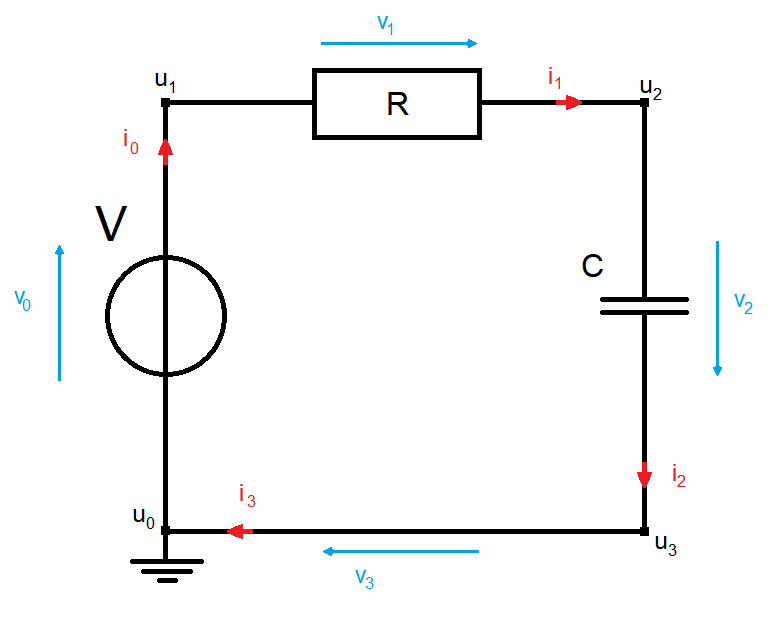
\includegraphics[scale=0.4]{../Tex/pictures/Example1_simple.png}
			\caption{charging capacitor with series resistor and voltage source}
			\label{circuit:charging of capacitor}
		\end{figure}
	\end{frame}

\section*{Formulating a Mathematical Model}

	\subsection{Network Topology}
		
	\begin{frame}
		\vfill
		Define the incidence matrix $A = (a_{ij}) \in \mathbb{R}^{k \times l}$:
		\begin{displaymath}
			\tilde{a}_{ij} = 
			\begin{cases}
				1 &   \text{edge $j$ starts at node $i$},\\
				-1 &  \text{edge $j$  ends at node $i$},\\
				0 & \text{else}.				
			\end{cases}
		\end{displaymath}
%		With 
%		\begin{align*}
%			\mathcal{N} = (n_0, n_1, n_2, ..., n_k) \quad &\cdots \quad \text{nodes},\\
%			\mathcal{E} = \{e_{j}: j = 1,...,l\} \quad &\cdots \quad \text{edges},
%		\end{align*}
%		furthermore
%		\begin{displaymath}
%			u = (u_0, u_1, u_2, ...) \quad \cdots \quad \text{corresponding electrical potentials at the nodes}.
%		\end{displaymath}
		By grounding node $0$, i.e. $u_0 = 0$ we obtain the reduced incidence matrix.
		\vfill
	\end{frame}

	\subsection{Energy Conservation Laws}
	\begin{frame}
		\vfill
		\begin{itemize}
			\item \textbf{Kirchhoff's voltage law (KVL):} \newline
			The sum of voltages along each loop of the network must equal to zero.
			\begin{equation}
				\label{KVL}
				\to A^\top  u = v.
			\end{equation}
			\item \textbf{Kirchhoff's current law (KCL):} \newline
			For any node, the sum of currents flowing into the node is equal to the sum of currents flowing out of the node.
			\begin{equation}
				\label{KCL}
				\to A  i = 0.
			\end{equation}
		\end{itemize}
		\vfill
	\end{frame}

	\subsection{Electrical Components and their Relations}
		
	\begin{frame}
		\begin{itemize}
			\item \textbf{Resistor} \newline
			\begin{equation}
				\label{eq:resistor law}
				v = R \ i \quad \text{or} \quad i = G \ u.
			\end{equation}
			\begin{figure}[H]
				\label{fig:resistor symbol}
				\centering
				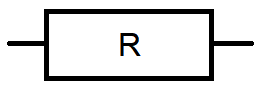
\includegraphics[width=2cm]{../Tex/pictures/resistor.png}
				\caption{resistor symbol}
			\end{figure}
			
			\item \textbf{Capacitor} \newline
			\begin{equation}
				\label{eq:capacitor law}
				Q = C \ v \quad \text{and by derivation in t} \quad I = C \ \frac{d}{dt}v = C \ v'.
			\end{equation}
			\begin{figure}[H]
				\label{fig:capacitor symbol}
				\centering
				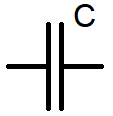
\includegraphics[width=2cm]{../Tex/pictures/capacitor.png}
				\caption{capacitor symbol}
			\end{figure}
		\end{itemize}
	\end{frame}
			
	\begin{frame}	
		\begin{itemize}
			\item \textbf{Inductor (Coil)} \newline
			\begin{equation}
				\label{eq:inductor law}
				\Phi = L \ i \quad \text{and by derivation in t} \quad v = L \ i'.
			\end{equation}
			\begin{figure}[H]
				\label{fig:inductor symbol}
				\centering
				
\includegraphics[width=3cm]{../Tex/pictures/inductance.png}
				\caption{inductor symbol}
			\end{figure}
			
			\item \textbf{Voltage Source} \newline
			\begin{equation}
				\label{eq:voltage source law}
				v = v_{src}
			\end{equation}
			\begin{figure}[H]
				\label{fig:voltage source symbol}
				\centering
				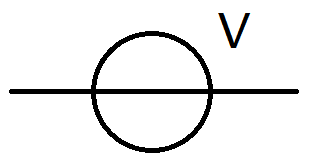
\includegraphics[width=4cm]{../Tex/pictures/voltage_source.png}
				\caption{voltage source symbol}
			\end{figure}
		\end{itemize}
	\end{frame}
			
	\begin{frame}
		\begin{itemize}
			\item \textbf{Current Source} \newline
			\begin{equation}
				\label{eq:current source law}
				i = i_{src}
			\end{equation}
			\begin{figure}[H]
				\label{fig:current source symbol}
				\centering
				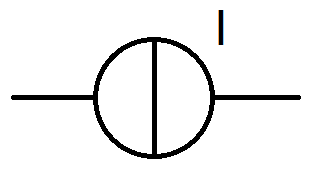
\includegraphics[width=4cm]{../Tex/pictures/current_source.png}
				\caption{current source symbol}
			\end{figure}
		\end{itemize}
	\end{frame}

	\subsection{Modified Nodal Analysis - MNA}
%	\begin{frame}
%		Rearrange the columns of the reduced incidence matrix $A$ into
%		\begin{displaymath}
%			A = (A_R A_C A_L A_V A_I)
%		\end{displaymath}
%		$A_R$, $A_C$, $A_L$, $A_V$ and $A_I$ ... columns related to components\\
%		Represent voltages:
%		\begin{displaymath}
%			v = A^\top u
%		\end{displaymath}
%		$\to$ rearrange $v$ into $v = (v_R, v_C, v_L, v_{src}, v_I)$ and $i$ into $i = (i_R, i_C, i_L, i_V, i_src)$. 
%		Rewrite component relations:
%		\begin{align*}
%			i_R = G \ v_R &= G \ A_R^\top u, \\
%			i_C = C \ v'_C &= C \ A_C^\top u'.
%		\end{align*}
%		Kirchhoffs current law:
%		\begin{displaymath}
%			A_C i_C + A_R i_R + A_L i_L + A_V i_V = -A_I i_{src}.
%		\end{displaymath}
%		Combine:
%		\begin{displaymath}
%			A_C C A_C^\top u' + A_R G A_R^\top u + A_L i_L + A_V i_V = -A_I i_{src}.
%		\end{displaymath}
%	\end{frame}

	\begin{frame}
%		Together with component law for inductors \eqref{eq:inductor law} and potential-voltage relation for voltage sources \eqref{eq:voltage source law}:
		Combining the component relations with the reduced incidence matrix and the Kirchhoff's laws we get:
		\begin{displaymath}
			\begin{aligned}
				A_C C A_C^\top u' + A_R G A_R^\top u + A_L i_L + A_V i_V &= - A_I i_{src} , \\
				L i_L'	- A_L^\top u &= 0 , \\
				-A_V^\top u &=  -v_{src}.
			\end{aligned}	
		\end{displaymath}
		In matrix form:
		\begin{equation}
			\label{MNA_Matrixform}
			\begin{pmatrix}
				A_C C A_C^\top & 0 & 0 \\
				0 & L & 0 \\
				0 & 0 & 0
			\end{pmatrix}
			*
			\begin{pmatrix}
				u' \\
				i_L' \\
				i_V'
			\end{pmatrix}
			+
			\begin{pmatrix}
				A_R G A_R^\top & A_L & A_V \\
				-A_L^\top & 0 & 0 \\
				-A_V^\top & 0 & 0 
			\end{pmatrix}
			*
			\begin{pmatrix}
				u \\
				i_L \\
				i_V
			\end{pmatrix}
			=
			\begin{pmatrix}
				-A_I i_{src} \\
				0 \\
				-v_{src}
			\end{pmatrix} . 
		\end{equation}
	\end{frame}

\section*{Differential Algebraic Equations}
	\subsection{Types of DAEs}
	\begin{frame}
		In the most general form a DAE can be written as:
		Find $y:\mathbb{R} \to \mathbb{R}^n$ such that
		\begin{equation}
			\label{Abstract_DAE}
			F(t, y(t), y'(t)) = 0, \qquad \forall t \in I
		\end{equation}
		
		with $F:\mathbb{R} \times \mathbb{R}^n \times \mathbb{R}^n \to \mathbb{R}^n$ sufficiently smooth and $I$ the time-interval.
		
		\textbf{Linear systems with constant coefficients} \newline
		find $y$ such that
		\begin{equation}
			\label{DAE-const-coeff}
			A y'(t) + B y(t) = f(t) ,
		\end{equation}
		with $A,B \in \mathbb{R}^{n \times n}$, $A$ singular, $B$ regular and $f:\mathbb{R} \to \mathbb{R}^n$ a function in time.
		
		\textbf{Linear time dependent systems}
		are systems of the form: find $y$ such that
		\begin{displaymath}
			A(t) y'(t) + B(t) y(t) = f(t) ,
		\end{displaymath}
		with $A, B:\mathbb{R} \to \mathbb{R}^{n \times n}$, $f:\mathbb{R} \to \mathbb{R}^n$ functions, $\forall t \in \mathbb{R}$: $A(t)$ is singular and $B(t)$ regular.
	\end{frame}
	
%	\begin{frame}
%		\begin{itemize}
%			\item \textbf{Linear systems with constant coefficients} \newline
%			find $y$ such that
%			\begin{equation}
%				\label{DAE-const-coeff}
%				A y'(t) + B y(t) = f(t) ,
%			\end{equation}
%			with $A,B \in \mathbb{R}^{n \times n}$, $A$ singular, $B$ regular and $f:\mathbb{R} \to \mathbb{R}^n$ a function in time.
%			
%			\item \textbf{Linear time dependent systems}
%			are systems of the form: find $y$ such that
%			\begin{displaymath}
%				A(t) y'(t) + B(t) y(t) = f(t) ,
%			\end{displaymath}
%			with $A, B:\mathbb{R} \to \mathbb{R}^{n \times n}$, $f:\mathbb{R} \to \mathbb{R}^n$ functions, $\forall t \in \mathbb{R}$: $A(t)$ is singular and $B(t)$ regular.
%			
%			\item  \textbf{Structured (non-linear) systems} \newline
%			are semi-explicit systems of the form: find $(y,z)$ such that
%			\begin{align}
%				y'(t) &= f(t, y(t), z(t)) , \\
%				0 &= g(t,y(t),z(t)) ,
%			\end{align}
%			with $f:\mathbb{R} \to \mathbb{R}^n$ and $g:\mathbb{R} \to \mathbb{R}^d$ functions.
%		\end{itemize}
%	\end{frame}

	\subsection{Weierstrass-Kronecker normalform}
	
	\begin{frame}
		prerequisites: \\
		\begin{definition}
			The matrix pencil $\{ A,B\}$ is called \emph{regular} if there exists some $c \in \mathbb{R}$, such that $(cA+B)$ is regular (i.e. $det(cA+B) \neq 0$), otherwise it is called singular.
		\end{definition}
%		\begin{theorem}[Jordan Normalform] %\protect{\cite[Theorem~13.2.1]{NumerikGewöhnlicherDifferentialgleichungen}}]
%			For every matrix $Q \in \mathbb{R}^{n \times n}$ there exists a regular matrix $T \in \mathbb{C}^{n \times n}$, such that
%			\begin{displaymath}
%				T^{-1}QT = J = diag(J_1, ..., J_r) \quad \text{with} \quad J_i = 
%				\left(
%				\begin{matrix}
%					\lambda_i & 1 & & 0 \\
%					0 & \lambda_i & \ddots & \vdots \\
%					& \ddots & \ddots & 1 \\
%					0 & \hdots & 0 & \lambda_i
%				\end{matrix}
%				\right)
%				\in \mathbb{C}^{m_i \times m_i}
%			\end{displaymath} 
%			and $n = m_1 + ... + m_r$.
%		\end{theorem}
	\end{frame}
	
%	\begin{frame}
%		\begin{theorem}[Weierstrass-Kronecker normalform]%[\protect{\cite[Satz~13.2.2]{NumerikGewöhnlicherDifferentialgleichungen}}]
%			\label{Kronecker-Normalform}
%			Let $\{ A,B \}$ be a regular matrix pencil. There exist $P,Q \in \mathbb{C}^{n \times n}$ such that
%			\begin{displaymath}
%				PAQ = 
%				\left(
%				\begin{matrix}
%					I_d & 0 \\
%					0 & N 
%				\end{matrix}
%				\right), \quad
%				PBQ = 
%				\left(
%				\begin{matrix}
%					R & 0 \\
%					0 & I_{n-d}
%				\end{matrix}
%				\right)
%			\end{displaymath}
%			where
%			\begin{displaymath}
%				N = diag(N_1, ..., N_r) \quad \text{with} \quad N_i = 
%				\left(
%				\begin{matrix}
%					0 & 1 & & 0\\
%					& \ddots &\ddots & \\
%					& & & 0 & 1 \\
%					0 & & & 0
%				\end{matrix}
%				\right)
%				\in \mathbb{R}^{n_i \times n_i}
%			\end{displaymath}
%			and R has Jordan Normalform. By $I_k$ we denote the identity matrix of size $k \times k$.
%		\end{theorem}
%		%Proof on blackboard
%	\end{frame}
	
	\begin{frame}
%		using these findings:
%		Using the findings above we are able to transform the initial DAE \eqref{DAE-const-coeff} using the matrix $P$ from Theorem \ref{Kronecker-Normalform}. By multiplying with $P$ from the left, we obtain
%		\begin{displaymath}
%			P A y'(t) + P B y(t) = P f(t) .
%		\end{displaymath}
%		
%		Setting
%		\begin{displaymath}
%			y(t) = Q
%			\left(
%			\begin{matrix}
%				u(t) \\
%				v(t)
%			\end{matrix}  
%			\right) 
%			, \quad
%			Pf(t) = 
%			\left(
%			\begin{matrix}
%				s(t) \\
%				q(t)
%			\end{matrix}
%			\right),
%		\end{displaymath}
%		with $u(t),s(t) : \mathbb{R} \to \mathbb{R}^d$ and $q(t),v(t) : \mathbb{R} \to \mathbb{R}^{n-d}$.
%		
		We get a system of the form
		\begin{equation}
			\label{transformed-DAE-const-coeff}
			\begin{aligned}
				u'(t) + Ru(t) &= s(t), \\
				Nv'(t) + v(t) &= q(t),
			\end{aligned}
		\end{equation}
		where $PAQ = 
		\left( 
		\begin{matrix}
			I & \\
			& N
		\end{matrix} 
		\right)$
		and $PBQ = 
		\left( 
		\begin{matrix}
			R & \\
			& I
		\end{matrix} 
		\right)$.
	\end{frame}
	
%	\begin{frame}
%		\begin{align}
%			\notag
%			v(t) &= q(t) - Nv'(t) = q(t) - N(\underbrace{q(t)-Nv'(t)}_{=v(t)})' = q-Nq'+N^2v'' \\ \notag
%			&= q-Nq'+N^2(q-Nv')'' = q-Nq'+N^2q''-N^3v''' \\ \notag
%			&\vdots \\ \notag
%			&= q-Nq'+...+(-1)^{k-1}N^{k-1}\underbrace{\frac{d^k}{dt^k}q}_{:=q^{(k-1)}}+(-1) \underbrace{N^kv^{(k)}}_{=0}\\ 
%			\label{solution-to-transformed-DAE-const-coeff-part2}
%			&= \sum_{i=0}^{k-1} (-1)^iN^iq^{(i)}(t)
%		\end{align}
%		where $k$ is the nilpotency index of $N$.
%	\end{frame}

	\begin{frame}
		\begin{definition}
			The nilpotency index $k$ of the matrix $N$ from the Weierstraß-Kronecker Normalform of a matrix pencil $\{A,B\}$ with $A$ singular is called the \emph{Kronecker-Index} of $\{A,B\}$, which we denote by $ind\{A,B\}$. Note that for $A$ regular we set $ind\{A,B\} = 0$.
		\end{definition}
	\end{frame}
	
	
	
	\subsection{Index of a Differential Algebraic Equation}
	
	\begin{frame}
		\begin{definition}%[differentiation index \protect{\cite[Definition~13.3.1]{NumerikGewöhnlicherDifferentialgleichungen}}]
			Consider the differential algebraic equation \eqref{Abstract_DAE} to be uniquely locally solvable and $F$ sufficiently smooth. For a given $m \in \mathbb{N}$ consider the equations
			\begin{displaymath}
				\begin{aligned}
					F(t,y,y') &= 0, \\
					\diff{F(t,y,y')}{t} &= 0, \\
					&\vdotswithin{=} \\
					\diff[m]{F(t,y,y')}{t} &= 0.
				\end{aligned}
			\end{displaymath}
			The smallest natural number $m$ for which the above system results in an explicit system of ordinary differential equations (ODEs), i.e. it has the form
			\begin{displaymath}
				y' = \phi(t,y),
			\end{displaymath}
			is called \textbf{differentiation index}.
		\end{definition}
	\end{frame}

	\begin{frame}
		\begin{definition}%[perturbation index \protect{\cite[Definition~13.3.3]{NumerikGewöhnlicherDifferentialgleichungen}}]
			Let $y(t)$ be the exact solution of \eqref{Abstract_DAE} and $\tilde{y}(t)$ be the solution of the perturbed system $F(t, \tilde{y}, \tilde{y}') = \delta(t)$. The smallest number $k \in \mathbb{N}$ such that 
			\begin{displaymath}
				\|y(t)-\tilde{y}(t)\| \leq C \left(\|y(t_0)-\tilde{y}(t_0)\|+\sum_{j=0}^{k}\max_{t_0 \leq \xi \leq T} \left\rVert 		\int_{t_0}^{\xi}\diff[j]{\delta}{\tau}(\tau)d \tau \right\rVert \right)
			\end{displaymath}
			for all $\tilde{y}(t)$, is called the \textbf{perturbation index} of this system.
		\end{definition}
	\end{frame}

\section*{Index Analysis of the Modified Nodal Analysis}
%	\subsection{General Index Analysis}
%	\begin{frame}
%		content...
%	\end{frame}
	\subsection{Topological Conditions}
	\begin{frame}
		\begin{theorem}[Index conditions] %\protect{\cite[Theorem~2.2.1]{shashkov_tuprints27452}}]
			Let the matrices of the capacitances, inductances and resistances be positive definite.
			\begin{itemize}
				\item If
				\begin{equation}
					\label{eq:index condition leq 2}
					ker([A_R, A_C, A_V, A_L]^\top) = \{0\} \quad \text{and} \quad ker(A_V) = \{0\}
				\end{equation}
				holds, then the MNA \eqref{MNA_Matrixform} leads to a system with index $\nu \leq 2$.
				
				\item If additionally
				\begin{equation}
					\label{eq:index condition leq 1}
					ker([A_R, A_C, A_V]^\top) = \{0\} \quad \text{and} \quad ker([A_C, A_V]) = \{0\}
				\end{equation}
				holds, then the system is of index $\nu \leq 1$
				
				\item If further
				\begin{equation}
					\label{eq:index condition eq 0}
					ker(A_C^\top) = \{0\} \quad \text{and} \quad dim(v_{src}) = 0
				\end{equation}
				holds, then the system has index $\nu = 0$.
			\end{itemize}
		\end{theorem}
	\end{frame}
	\begin{frame}
		\begin{itemize}
			\item Condition \eqref{eq:index condition leq 2} can be interpreted, as the circuit neither containing loops of voltage sources nor cutsets of current sources.
			\item Condition \eqref{eq:index condition leq 1} can be interpreted, as the circuit containing neither loops of capacitors and/or voltage sources nor cutsets of inductors and/or current sources.
			\item Condition \eqref{eq:index condition eq 0} can be interpreted, as every node in the circuit being connected to the reference node (ground) through a path containing only the capacitors.
		\end{itemize}
	\end{frame}

\section*{Numerical Solutions}
%	\begin{frame}
%		general initial value problem
%		Find y, such that
%		\begin{align}
%			\label{general numerical problem}
%			y'(t) &= f(t,y), \quad t \in [t_0, t_l], \\
%			y(t_0) &= y_0.
%		\end{align}
%		
%		\begin{figure}[H]
%			\centering
%			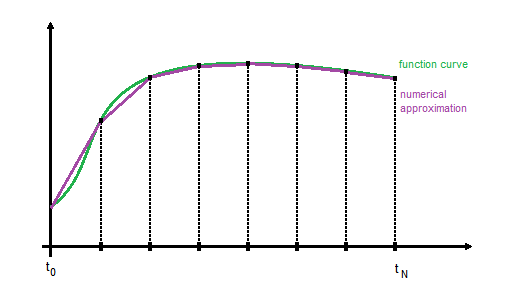
\includegraphics[scale=0.7]{../Tex/pictures/num_approx.png}
%			\caption{approximation of a function using numerical methods}
%			\label{fig:numerical approximation}
%		\end{figure}
%		
%	\end{frame}
%	\subsection{Single-Step Methods}
%	\begin{frame}
%		\begin{definition}
%			\label{def:single step mehod}
%			A numerical method to approximate a differential equation \ref{general numerical problem} on a time-grid $t_0,...,t_l$ with the intermediate values $y_0,...,y_l$ is called a single-step method if it is of the form
%			\begin{equation}
%				\label{single-step method}
%				y_{j+1} = y_j + h_j \phi(t_j,y_j, y_{j+1},h_j).
%			\end{equation}
%			We call $\phi$ the \emph{procedural function}. If $\phi$ does not depend on $y_{j+1}$, then the method is called \emph{explicit}, otherwise it is called \emph{implicit}.
%		\end{definition}
%	\end{frame}
	
%	\subsubsection{Consistency, Stability and Convergence}
%	\begin{frame}
%		\begin{definition}\label{Discretization_Error_SingleStep}
%			Let $y_{m+1}$ be the result of one step of a single step method \eqref{single-step method} with the exact start-vector $y_m = y(t_m)$ then
%			\begin{equation}
%				\label{local discretization error single step}
%				\delta_{m+1} = \delta(t_m+h) = y(t_{m+1}) - \tilde{y}_{m+1}, \quad m = 0,...,N-1
%			\end{equation}
%			is called the \emph{local discretization error} of the single step method at the point $t_{m+1}$.
%		\end{definition}
%	\end{frame}
%	
%	\begin{frame}
%		\begin{definition}\label{Consistency_SingleStep}
%			A single-step method is called \emph{consistent} if for all initial value problems \eqref{general numerical problem} 
%			\begin{equation}
%				\lim\limits_{h \to 0} \frac{\|\delta(t+h)\|}{h} = 0 \quad \text{for} \quad t_0 \leq t \leq t_l
%			\end{equation}
%			holds.\newline
%			It is called \emph{consistent of order p}, if for a sufficiently smooth function $f$
%			\begin{equation}
%				\|\delta(t+h)\| \leq Ch^{p+1} \quad \text{for all} \quad h \in \mathopen{(} 0,H \mathclose{]} \quad \text{and} \quad t_0 \leq t \leq t_l - h
%			\end{equation}
%			holds with $C$ independent of $h$.
%		\end{definition}
%	\end{frame}
%	
%	\begin{frame}
%		\begin{definition}\label{Convergence_SingleStep}
%			A single-step method is called \emph{convergent}, if for all initial value problems \eqref{general numerical problem} for the \emph{global discretization error}
%			\begin{displaymath}
%				e_m = y(t_m)-y_m
%			\end{displaymath}
%			holds that
%			\begin{displaymath}
%				\max\limits_{m}\|e_m\| \to 0 \quad \text{for} \quad h_{max} \to 0.
%			\end{displaymath}
%			The single-step method is called to have the \emph{convergence order} $p$, if
%			\begin{displaymath}
%				\max\limits_{m} \|e_m\| \leq C h_{max}^p \quad \text{for} \quad h_{max} \in \mathopen{(} 0,H \mathclose{]} \quad \text{with} \quad t_0 \leq t_m \leq t_l
%			\end{displaymath}
%			with the constant $C$ not dependent on the step size $h$.
%		\end{definition}
%	\end{frame}
%	
%	\begin{frame}
%		\begin{definition}\label{Discrete_Stability_SingleStep - lecture notes for numpdgl}
%			A single-step method is called \emph{(discretely) stable} if for grid-functions $y_h$ and $\tilde{y}_h$ with
%			\begin{align}
%				y_{i+1} &= y_i + h \phi(t_i, y_i), \\
%				\tilde{y}_{i+1} &=  \tilde{y}_i + h [\phi(t_i, \tilde{y}_i) + \theta_i],
%			\end{align}
%			and perturbations $\theta_i = \theta_h(t_i)$ of the right side as well as a bounded perturbation in the initial-values $y_0 - \tilde{y}_0$ the error is bounded by
%			\begin{displaymath}
%				\|y_h - \tilde{y}_h\|_{\infty,h} \leq C (\|y_0 - \tilde{y}_0\|_{l^2} + \|\theta_h\|_{\infty,h})
%			\end{displaymath}
%			with a constant $C$ which is not dependent on $h$. The norm $\|.\|_{\infty,h}$ denotes the maximum norm over the time-grid, i.e. for a function $b: T={t_0,...,t_N} \to \mathbb{R}^d$ we have $\|b\|_{\infty,h} = \max\limits_{t \in T}\|b(t)\|$, $\|b\|$ is the euclidean norm.
%		\end{definition}
%	\end{frame}
%	
%	\subsubsection{further stability properties}
%	
%	\begin{frame}
%		 Dahlquist equation, i.e. find $y$ such that
%		\begin{align}
%			y' &= \lambda y, \quad t > 0 \\
%			y(0) &= y_0
%		\end{align}
%		with $\lambda \in \mathbb{C}$ and $u_0$ fixed.
%	\end{frame}
%	
%	\begin{frame}
%		\begin{definition}
%			\begin{enumerate}
%				\item 
%				If a single-step method can be written in the form
%				\begin{equation}
%					y_{i+1} = R(z) \ y_i, \quad z:= h \lambda
%				\end{equation}
%				then we call $R: \mathbb{C} \to \mathbb{C}$ the \emph{stability function} of the single-step method.
%				\item 
%				The set
%				\begin{equation}
%					S := \{z \in \mathbb{C} : |R(z)| \leq 1\}
%				\end{equation}
%				is called the \emph{region of stability} of the method.
%				\item 
%				A single-step method is called
%				\begin{itemize}
%					\item \emph{0-stable}, if $0 \in S$.
%					\item \emph{A-stable}, if $\mathbb{C}^- \subset S$.
%					\item \emph{L-stable}, if $R(z) \to 0$ for $Re(z) \to -\infty$.
%				\end{itemize}
%			\end{enumerate}
%		\end{definition}
%	\end{frame}
	
	\subsection{Multistep Methods}
	\begin{frame}
		\begin{definition}
			\label{def:multi step method}
			For given $\alpha_0, ..., \alpha_k$ and $\beta_0, ..., \beta_k$ the iteration rule
			\begin{equation}
				\label{linear-multistep-method}
				\sum_{l=0}^{k} \alpha_l y_{m+l} = h \sum_{l=0}^{k} \beta_l f(t_{m+l}, y_{m+l}), \quad m=0,1,...,N-k
			\end{equation}
			is called a \emph{linear multistep method} (linear k-step method). It is always assumed that $\alpha_k \neq 0$ and $|\alpha_0| + |\beta_k| > 0$. If $\beta_k=0$ holds, then the method is called explicit, otherwise implicit.
		\end{definition}
	\end{frame}
	
%	\subsubsection{Consistency, Convergence and Stability}
%	
%	\begin{frame}
%		\begin{definition}
%			Let $y_{m+k}$ be the result of one step of the multi-step method \eqref{linear-multistep-method} with the start-values given as the evaluations of the exact solution $y_{m+l} = y(t_{m+l})$ at $0 \leq l < k$. This means
%			\begin{displaymath}
%				\alpha_k \tilde{u}_{m+k} = \sum_{l=0}^{k-1} \left( h \beta_l f(t_{m+l}, y(t_{m+l})) - \alpha_l y(t_{m+l}) \right) + h \beta_k f(t_{m+k}, y_{m+k}) .
%			\end{displaymath}
%			Then
%			\begin{displaymath}
%				\delta_{m+k} = \delta(t_{m+k}) = y(t_{m+k}) - y_{m+k}, \quad m=0,1,...,N-k
%			\end{displaymath}
%			is called the \emph{local discretization error} (local error) of the linear multi-step method, see Def. \ref{linear-multistep-method} at the point $t_{m+k}$.
%		\end{definition}
%	\end{frame}
%	
%	\begin{frame}
%		\begin{definition}
%			A linear multi-step method is called %\emph{preconsistent} if for all functions $y(t) \in C^1[t_0,t_l]$
%			%		\begin{displaymath}
%				%			\lim\limits_{h \to 0} L[y(t),h]=0
%				%		\end{displaymath}
%			%		holds. 
%			%		It is called 
%			\emph{consistent}, if for all functions $y(t) \in C^2([t_0,t_l])$
%			\begin{displaymath}
%				\lim\limits_{h \to 0} \frac{1}{h} L[y(t),h] = 0
%			\end{displaymath}
%			holds. It has the \emph{consistency order p}, if for all functions $y(t) \in C^{p+1}[t_0, t_l]$
%			\begin{displaymath}
%				L[y(t),h] = \mathcal{O}(h^{p+1}) \quad \text{for} \quad h \to 0
%			\end{displaymath}
%			holds.
%		\end{definition}
%	\end{frame}
	
	\begin{frame}
		\begin{definition} \label{def: LMSM convergence}
			We say that a linear multi-step method is convergent if for a solution $y$ of the problem a solution vector created by an LMSM $y_j$ for $j \in {0,...,k}$ we have that
			\begin{displaymath}
				\lim\limits_{h \to \infty} \max_{0 \leq j \leq k} ||y(t_j) - y_j|| = 0.
			\end{displaymath}
		\end{definition}
	\end{frame}
	
%	\begin{frame}
%		\begin{definition} \label{discrete stability LMSM}
%			A linear multi-step method is called (discretely) stable, if for solutions $y_h$ and $\tilde{y}_h$ of
%			\begin{align}
%				\sum_{l=0}^{k} \alpha_l y_{m+l} &= h \sum_{l=0}^{k} \beta_l f(t_{m+l}, y_{m+l}), \\
%				\sum_{l=0}^{k} \alpha_l \tilde{y}_{m+l} &= h \sum_{l=0}^{k} \beta_l f(t_{m+l}, \tilde{y}_{m+l}) + h\theta_n
%			\end{align} 
%			and bounded initial values $y_j - \tilde{y}_j$ for $j \in {0,...,k}$ we have that
%			\begin{displaymath}
%				\max_{t_0 \leq t_n \leq T} ||y_n - \tilde{y}_n|| \leq C \sum_{j=0}^{k-1} ||y_j - \tilde{y}_j|| + \max_{t_0 \leq t_n \leq T} ||\theta_n||.
%			\end{displaymath}
%		\end{definition}
%	\end{frame}
	
	\subsubsection{further stability properties}
	
	\begin{frame}
		Dahlquist test problem as a model problem, find $y$ such that
		\begin{align}
			y' &= \lambda y, \quad t > 0 \\
			y(0) &= y_0
		\end{align}
		with $\lambda \in \mathbb{C}$ and $y_0$ fixed. \\
		Thus the resulting linear multistep method is of the form
		\begin{align*}
			\sum_{l=0}^{k} \alpha_l y_{n+l} = h \sum_{l=0}^{k} \beta_l \lambda y_{n+l} \\
			\iff \sum_{l=0}^{k}  [\alpha_l - h \beta_l \lambda] y_{n+l}
		\end{align*}
	\end{frame}
	
	\begin{frame}
			\begin{definition}
			\begin{enumerate}
				\item 
				The set
				\begin{equation}
					\begin{aligned}
						S := \{z \in \mathbb{C} : \rho(\xi) - z \sigma(\xi) = 0 \implies \xi \in \mathbb{C} \text{ and } |\xi| \leq 1. \\
						\text{ If $\xi$ has multiplicity greater than $1$, then } |\xi| < 1\}
					\end{aligned}
				\end{equation}
				is called the region of stability of the method.
				\item 
				A linear multistep method is called
				\begin{itemize}
					\item \emph{0-stable}, if $0 \in S$.
					\item stable in the point $z \in \mathbb{C}$, if $z \in S$.
					\item \emph{$A(\alpha)$-stable}, if it is stable in all $z$ that lie within the set $\{z \in \mathbb{C}^- : |arg(z)-\pi| \leq \alpha\}$ for $\alpha \in (0, \frac{\pi}{2})$.		 
				\end{itemize}
			\end{enumerate}
		\end{definition}
	\end{frame}
	
	\begin{frame}
		\begin{theorem}%[\protecting{\cite[Satz~4.2.10]{NumerikGewöhnlicherDifferentialgleichungen}}]
			\label{th: null-stbaility and consistence is convergence}
			Let $f(t,y)$ be sufficiently smooth and the linear multi-step method be zero-stable and consistent of order $p$, then it is also convergent of order $p$.
		\end{theorem}
	\end{frame}
	
	\subsection{Consistent Initial Values}
	\begin{frame}
		index $\nu = 0$.\\ 
		
		Case: Index $\nu = 1$.\\
		
		By rewriting our system into the form
		
		\begin{align*}
			y'(t) = f(t,y(t),z(t)), \\
			0 = g(t,y(t),z(t)).
		\end{align*}
		
		we are able to give conditions for consistent initial values. Namely $y_0$ and $z_0$ are consistent initial values for this system, if $g(t_0, y_0, z_0) = 0$ holds.
		
	\end{frame}
	
	\begin{frame}
		Case: Index $\nu = 2$.\\
		
		For index-2 systems we rewrite our system into
		
		\begin{align*}
			y' = f(t,y(t),z(t)), \\
			0 = g(t,y(t)).
		\end{align*}
		
		Consistent initial values $y_0$, $z_0$ for this case not only have to fulfill $g(t_0, y_0) = 0$ but also the \emph{hidden constraint} $g_t(t_0, y_0) + g_y(t_0, y_0)f(t_0, y_0, z_0)$. By $g_t$ and $g_y$ we denote the derivative of $g$ with respect to $t$ or $y$, respectively.
	\end{frame}
	
	\subsection*{Implicit Linear Multistep Formulas}
	
	\subsubsection{BDF-k Methods}
	
	\begin{frame}
		The \emph{backward differentiation formula (BDF)} is a family of implicit linear multistep methods. They have the general form
		\begin{equation}
			\sum_{k=0}^{s} \alpha_k y_{n+k} = h \beta f(t_{n+s}, y_{n+s})
		\end{equation}
		The BDF or BDF-k formulas for $k=1,...,3$ have the following form %or till 6
		\begin{align*}
			k = 1 &: h f_{m+1} = y_{m+1} - y_m \\
			k = 2 &: h f_{m+2} = \frac{1}{2} (3 y_{m+2} - 4 y_{m+1} + y_m) \\
			k = 3 &: h f_{m+3} = \frac{1}{6} (11 y_{m+3} - 18 y_{m+2} + 9 y_{m+1} - 2 y_m) %\\
			%		k = 4 &: h f_{m+4} = \frac{1}{12} (25 u_{m+4} - 48 u_{m+3} + 36 u_{m+2} - 16 u_{m+1} + 3 u_m) \\
			%		k = 5 &: h f_{m+5} = \frac{1}{260} (137 u_{m+5} - 300 u_{m+4} + 300 u_{m+3} - 200 u_{m+2} +75 u_{m+1} -12 u_m) \\
			%		k = 6 &: h f_{m+6} = \frac{1}{60} (147 u_{m+6} - 360 u_{m+5} + 450 u_{m+4} - 400 u_{m+3} + 225 u_{m+2} - 72 u_{m+1} + 10 u_m)
		\end{align*}
	\end{frame}
	
	\begin{frame}
		\begin{figure}[H]
			\centering
			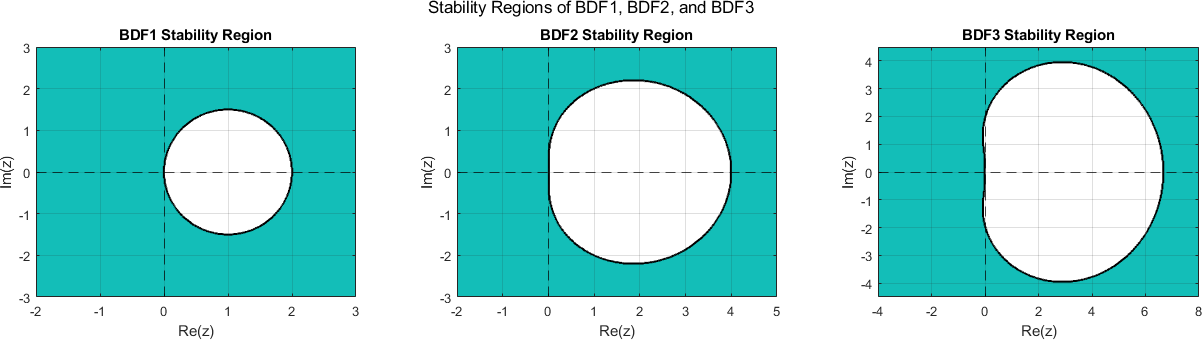
\includegraphics[width=1\linewidth]{../Tex/pictures/bdf_stability_regions.png}
			\caption{stability regions of BDF-schemes}
			\label{fig:screenshot020}
		\end{figure}
		\begin{theorem}%[\protecting{\cite[Satz~9.2.1]{NumerikGewöhnlicherDifferentialgleichungen}}]
			The BDF-k methods have consistency order $p=k$.
		\end{theorem}
	\end{frame}
	
	\subsubsection{Trapezoidal rule}
	
	\begin{frame}
		This procedure is repeated for small subsections of the interval $[a,b]$. Thus we obtain the iteration formula
		\begin{displaymath}
			u_h (t+h) = u_h(t) +\frac{h}{2}[f(t,u_h(t)) + f(t+h, u_h(t+h))].
		\end{displaymath}
	\end{frame}
	
	\subsection*{Numerical Examples}
	
	\subsubsection{Example1}
	
	\begin{frame}
		\begin{figure}[H]
			\centering
			\begin{minipage}{.5\textwidth}
				\centering
				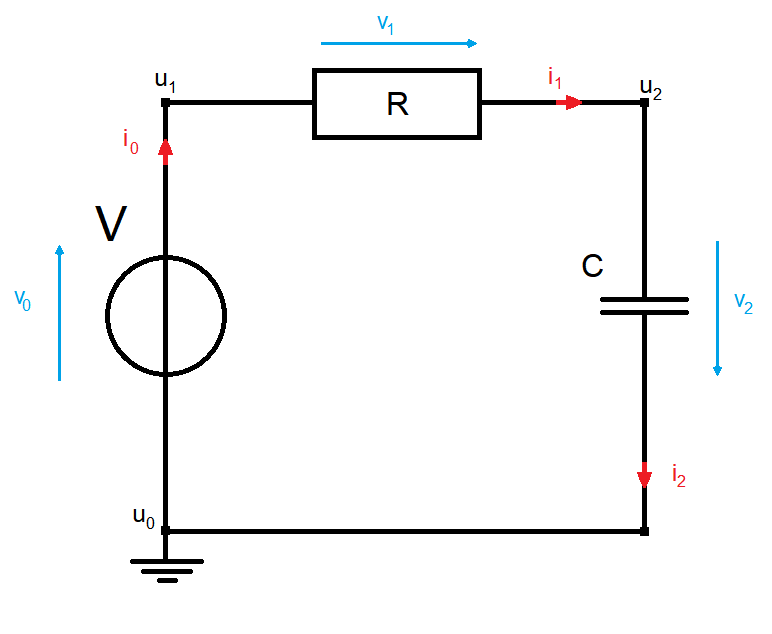
\includegraphics[width=\linewidth]{../Tex/pictures/Example1_simple_p2.png}
				\caption{charging capacitor with series resistor and voltage source}
				\label{fig:charging capacitor}
			\end{minipage}%
			\begin{minipage}{.5\textwidth}
				\centering
				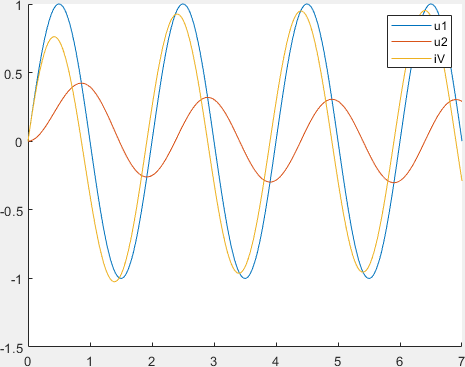
\includegraphics[width=\linewidth]{../Tex/pictures/exact_solution_ex1.png}
				\caption{Exact solution for example 1.}
				\label{fig: Exact solution for example 1}
			\end{minipage}
		\end{figure}
	\end{frame}
	
	\begin{frame}
		\begin{table}[H]
			\resizebox*{\textwidth}{!}{%
				\csvreader[tabular= | c || c c | c c | c c | c c |,
				table head = \hline h & \multicolumn{2}{c|}{k = 1} & \multicolumn{2}{c|}{k = 2} & \multicolumn{2}{c|}{k = 3} & \multicolumn{2}{c|}{trapezoidal}\\
				& u2 & iV & u2 & iV & u2 & iV & u2 & iV \\
				\hline,
				late after line=\\\hline]
				{../Matlab/err_ex1.csv}{h=\h, oneu=\oneu, oneuu=\oneuu, onei=\onei, twou=\twou, twouu=\twouu, twoi=\twoi, threeu=\threeu, threeuu=\threeuu, threei=\threei, trapu=\trapu, trapuu=\trapuu, trapil=\trapil}
				{\h  & \num{\oneuu} & \num{\onei}  & \num{\twouu} & \num{\twoi}  & \num{\threeuu} & \num{\threei}  & \num{\trapuu} & \num{\trapil}}
			}
			\caption{Resulting errors for the BDF-k methods and ther trapezoidal rule.}
			\label{tab:num results ex1}
		\end{table}
	\end{frame}
	
%	\subsubsection{Example 2}
%	
%	\begin{frame}
%		\begin{figure}[H]
%			\centering
%			\begin{minipage}{.5\textwidth}
%				\centering
%				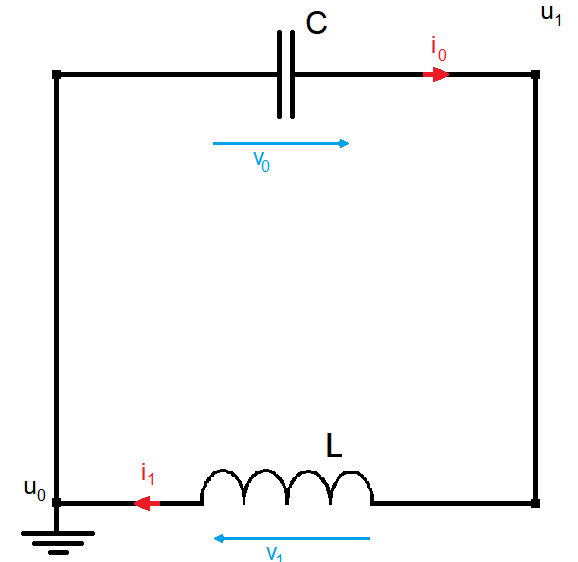
\includegraphics[width=\linewidth]{../Tex/pictures/Example2_index0.png}
%				\caption{LC-circuit}
%				\label{fig: LC-circuit}
%			\end{minipage}%
%			\begin{minipage}{.5\textwidth}
%				\centering
%				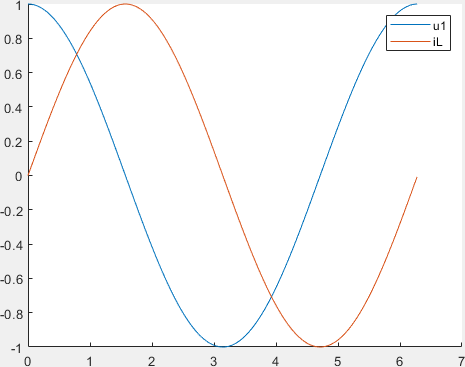
\includegraphics[width=\linewidth]{../Tex/pictures/exact_solution_ex2.png}
%				\caption{Exact solution for example 2.}
%				\label{fig: Exact solution for example 2}
%			\end{minipage}
%		\end{figure}
%	\end{frame}
%	
%	\begin{frame}
%		\begin{table}[H]
%			\resizebox*{\textwidth}{!}{%
%				\csvreader[tabular= | c || c c | c c | c c | c c | ,
%				table head = \hline h & \multicolumn{2}{c|}{k = 1} & \multicolumn{2}{c|}{k = 2} & \multicolumn{2}{c|}{k = 3} & \multicolumn{2}{c|}{trapezoidal} \\
%				& u1 & iL & u1 & iL & u1 & iL & u1 & iL \\
%				\hline,
%				late after line=\\\hline]
%				{../Matlab/err_ex2.csv}{h=\h, oneu=\oneu, onei=\onei, twou=\twou, twoi=\twoi, threeu=\threeu, threei=\threei, trapu=\trapu, trapil=\trapil}
%				{\h & \num{\oneu} & \num{\onei} & \num{\twou} & \num{\twoi} & \num{\threeu} & \num{\threei} & \num{\trapu} & \num{\trapil}}
%			}
%			\caption{Resulting errors for the BDF-k methods and ther trapezoidal rule.}
%			\label{tab:error ex2}
%		\end{table}
%	\end{frame}
%	
%	\subsubsection{Example 3}
%	
%	\begin{frame}
%		\begin{figure}[H]
%			\centering
%			\begin{minipage}{.5\textwidth}
%				\centering
%				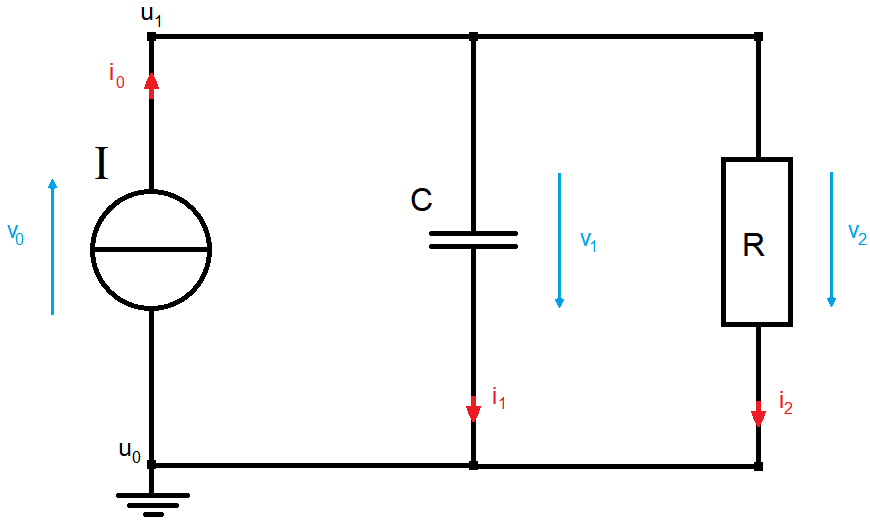
\includegraphics[width=\linewidth]{../Tex/pictures/Example3.png}
%				\caption{Current source with capacitor and resistor.}
%				\label{fig:num ex3}
%			\end{minipage}%
%			\begin{minipage}{.5\textwidth}
%				\centering
%				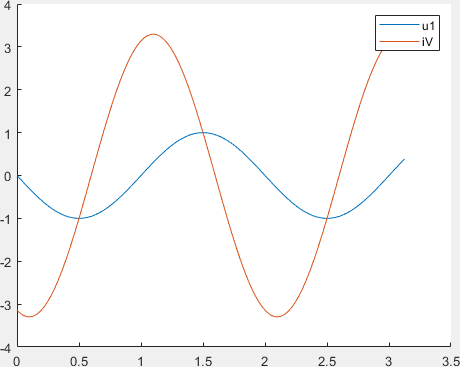
\includegraphics[width=\linewidth]{../Tex/pictures/exact_solution_ex3.png}
%				\caption{Exact solution for example 3.}
%				\label{fig: Exact solution for example 3}
%			\end{minipage}
%		\end{figure}
%	\end{frame}
%	
%	\begin{frame}
%		\begin{table}[H]
%			%\resizebox*{\textwidth}{!}{%
%				\centering
%				\csvreader[tabular= | c || c | c | c | c | ,
%				table head = \hline h & {k = 1} & {k = 2} & {k = 3} & trapezoidal \\ %\multicolumn{1}{c|}{}
%				& iV & iV & iV & iV \\
%				\hline,
%				late after line=\\\hline]
%				{../Matlab/err_ex3.csv}{h=\h, oneu=\oneu, onei=\onei, twou=\twou, twoi=\twoi, threeu=\threeu, threei=\threei, trapu=\trapu, trapil=\trapil}
%				{\h & \num{\onei} & \num{\twoi} & \num{\threei} & \num{\trapil}}
%				%}
%			\caption{Resulting errors for the BDF-k methods and the trapezoidal rule.}
%			\label{tab:error ex3}
%		\end{table}
%	\end{frame}












%\section{Getting Started}
%
%\begin{frame}[containsverbatim]
%\frametitle{Getting Started}
%
%\begin{itemize}
%\item Begin your new presentation with \verb|\documentclass[<class options>]{beamer}|, where \verb|<class options>| is a comma-separated list of options:
%    \begin{itemize}
%    \item A typical class option is \verb|aspectratio=169| to set the slide aspect ratio to 16:9. Use \verb|aspectratio=43| to set the slide aspect ratio to 4:3.
%    \item You should define at least one document language, e.g.\ \verb|english| or \verb|ngerman| (the ``n'' is intended). The last language will become the document default language.
%    \item When you use pdfLaTeX, always add the option \verb|utf8| so that input files are treated as UTF-8 encoded.
%    \end{itemize}
%
%\item Next, select the JKU beamer theme with \verb|\usetheme[<theme options>]{jku}| (\verb|<theme options>| is, again, a comma-separated list of options).
%\end{itemize}
%\end{frame}
%
%
%\subsection{Theme Options}
%
%\begin{frame}[containsverbatim,label={options:colorscheme}]
%\frametitle{Theme Options: Selecting a Color Scheme}
%%\begin{table}
%    \begin{tabularx}{\linewidth}{ll>{\raggedright}X}
%    \toprule
%    \textbf{Option} & \textbf{Color Scheme} & \textbf{Primary Color} \tabularnewline
%    \midrule
%    \textverb{JKU}    & JKU (gray) scheme                   & \mbox{\usebeamercolor[fg]{palette jku}\rule{6em}{10pt}} \tabularnewline
%    \textverb{BUS}    & Business School scheme              & \mbox{\usebeamercolor[fg]{palette bus}\rule{6em}{10pt}} \tabularnewline
%    \textverb{LIT}    & Linz Institute of Technology scheme & \mbox{\usebeamercolor[fg]{palette lit}\rule{6em}{10pt}} \tabularnewline
%    \textverb{MED}    & MED faculty scheme                  & \mbox{\usebeamercolor[fg]{palette med}\rule{6em}{10pt}} \tabularnewline
%    \textverb{RE}     & RE faculty scheme                   & \mbox{\usebeamercolor[fg]{palette re}\rule{6em}{10pt}} \tabularnewline
%    \textverb{SOE}    & School of Education scheme          & \mbox{\usebeamercolor[fg]{palette soe}\rule{6em}{10pt}} \tabularnewline
%    \textverb{SOWI}   & SOWI faculty scheme                 & \mbox{\usebeamercolor[fg]{palette sowi}\rule{6em}{10pt}} \tabularnewline
%    \textverb{TNF}    & TNF faculty scheme                  & \mbox{\usebeamercolor[fg]{palette tnf}\rule{6em}{10pt}} \tabularnewline
%    \bottomrule
%    \end{tabularx}
%%\end{table}
%
%\smallskip
%If no color scheme option is given, the package defaults to using \texttt{JKU}.
%\end{frame}
%
%
%\begin{frame}[containsverbatim,label={options:colormode}]
%\frametitle{Theme Options: Selecting a Color Mode}
%\begin{itemize}
%\item The theme uses light color mode by default. In this color mode, all frames (including title, logo, and section frames) have a white background.
%\item Use option ``\verb|darkmode|'' to display title, logo, and section frames with a dark background (primary color of the current color scheme).
%\end{itemize}
%\end{frame}
%
%
%\begin{frame}[containsverbatim,label={options:slide-numbers}]
%\frametitle{Theme Options: Slide Numbers}
%No slide numbers are shown in slide footers by default. Enable them with:
%
%\smallskip
%%\begin{table}
%    \begin{tabularx}{\linewidth}{l>{\raggedright}X}
%    \toprule
%    \textbf{Option}                & \textbf{Description} \tabularnewline
%    \midrule
%    \textverb{framenumber}         & Insert slide number into the footer. \tabularnewline
%    \textverb{totalframenumber}    & Insert slide number and total slide number into the footer. \tabularnewline
%    \textverb{appendixframenumber} & Like ``\textverb{totalframenumber}'', but also count slides from the appendix into the total. Combine with ``\textverb{totalframenumber}'' to only show the overall total for appendix slides. \tabularnewline
%    \bottomrule
%    \end{tabularx}
%%\end{table}
%
%\smallskip
%Btw., if you want to reference a slide number, use the option \verb+[label={s}]+ in the target frame. Then \verb+\ref{s}+ will give a reference to the slide number. For instance, slide~\ref{options:section-slides} is the next slide.
%\end{frame}
%
%
%\begin{frame}[containsverbatim,label={options:section-slides}]
%\frametitle{Theme Options: Section Slides}
%By default, each sectioning command (\verb|\section|, \verb|\subsection|, \verb|\subsubsection|) inserts a section slide. You can globally disable section slides with:
%
%\smallskip
%%\begin{table}
%    \begin{tabularx}{\linewidth}{l>{\raggedright}X}
%    \toprule
%    \textbf{Option}            & \textbf{Description} \tabularnewline
%    \midrule
%    \textverb{nosectionpage}       & Supress all section slides. \tabularnewline
%    \textverb{nosubsectionpage}    & Supress subsection and subsubsection slides. \tabularnewline
%    \textverb{nosubsubsectionpage} & Supress subsubsection slides. \tabularnewline
%    \bottomrule
%    \end{tabularx}
%%\end{table}
%
%\smallskip
%\begin{itemize}
%\item The class option \verb|handout| also supresses these slides but includes them in slide numbering.
%\item The starred versions of sectioning commands (e.g.\ \verb|\section*{...}|) also supress section slides. 
%\end{itemize}
%\end{frame}
%
%
%\begin{frame}[containsverbatim]
%\frametitle{More Theme Options}
%%\begin{table}
%    \begin{tabularx}{\linewidth}{l>{\raggedright}X}
%    \toprule
%    \textbf{Option}			     & \textbf{Description} \tabularnewline
%    \midrule
%    \textverb{compactmono}         & Use condensed fixed-width font everywhere. \tabularnewline
%    \textverb{nocompactverb}       & Do not use condensed fixed-width font for verbatim and listings. \tabularnewline
%    \textverb{nofooter}            & Supress slide footer. \tabularnewline
%    \textverb{nojkufooter}         & Supress JKU/partner logos in slide footer. \tabularnewline
%    \textverb{noimprint}           & Supress imprint on title slides. \tabularnewline
%    \textverb{nooptpackages}       & Do not load additional convenience packages (which are only there to provide interoperability to the behavior of previous versions of this theme but are not actually required for the current version). \tabularnewline
%    \bottomrule
%    \end{tabularx}
%%\end{table}
%\end{frame}
%
%
%\subsection{Title Slide \& Slide Footers}
%
%\begin{frame}[containsverbatim]
%\frametitle{Title Slide}
%
%Use \verb+\maketitle+ to display a title slide. This command uses the following information:
%
%\smallskip
%%\begin{table}
%    \begin{tabularx}{\linewidth}{l>{\raggedright}X}
%    \toprule
%    \textbf{Command}                    & \textbf{Description} \tabularnewline
%    \midrule
%    \textverb{\string\title\{...\}}     & The title of your presentation. \tabularnewline
%    \textverb{\string\subtitle\{...\}}  & The subtitle of your presentation. \tabularnewline
%    \textverb{\string\author\{...\}}    & The speakers / authors of the presentation.
%                                          % Use \textverb{\string\and} to separate multiple author names. 
%                                          \tabularnewline
%    \textverb{\string\institute\{...\}} & The intitute / affiliations of the author(s). \tabularnewline
%    \textverb{\string\date\{...\}}      & The date of the presentation. Defaults to today's date if omitted. Use \textverb{\string\date\{\}} to supress the date. \tabularnewline
%    \bottomrule
%    \end{tabularx}
%%\end{table}
%
%\smallskip
%\small An optional argument (\verb|\cmd[opt]{...}|) allows to set short versions for use in e.g.\ footers.
%\end{frame}
%
%
%\begin{frame}[containsverbatim,label={advanced-title-slides}]
%\frametitle{Advanced Title Slides}
%
%\begin{itemize}
%\item You can change the presentation information and use the \verb+\maketitle+ command multiple times in your presentation.
%\item An optional argument \verb|\maketitle[<options>]| allows to change the color scheme of the title slide. Options may be one of:
%    \begin{itemize}
%    \item \textverb{light}: Use light color theme.
%    \item \textverb{dark}: Use dark color theme.
%    \item \textverb{gray}: Use JKU gray color theme.
%    \item \textverb{black}: Use black background.
%    \end{itemize}
%    In addition, options may contain a faculty name (see \hyperref[options:colorscheme]{Theme Options: Selecting a Color Scheme}) to use the faculty's color theme, e.g. ``\verb|\maketitle[TNF,dark]|''.
%\end{itemize}
%\end{frame}
%
%\title{Space for new title}
%\subtitle{Space for new subtitle}
%\maketitle[TNF,dark]
%
%
%\begin{frame}[containsverbatim]
%\frametitle{Logos}
%
%%\begin{table}
%    \begin{tabularx}{\linewidth}{l>{\raggedright}X}
%    \toprule
%    \textbf{Command}                           & \textbf{Description} \tabularnewline
%    \midrule
%    \textverb{\string\institutecode\{code\}}   & The abbreviation / initials of the institute. Use this to load your institute logo instead of the standard JKU logo. E.g.\ \textverb{\string\institutecode\{LIT\}} to load the LIT logo. You need to add your logo files to the logos folder. \tabularnewline
%    \textverb{\string\partnerlogo\{filename\}} & The logo of a partner institution. \textverb{filename} must point to an image file. File extension may be omitted. \tabularnewline
%    \textverb{\string\footerpartnerlogo\{...\}} & Change the partner logo in the footer. Use this only if you need to display a different partner logo file (e.g.\ with a different geometry) in the footer. \tabularnewline
%    \bottomrule
%    \end{tabularx}
%%\end{table}
%\end{frame}
%
%
%\begin{frame}[containsverbatim]
%\frametitle{Customizing the Slide Footer}
%
%%\begin{table}
%    \begin{tabularx}{\linewidth}{l>{\raggedright}X}
%    \toprule
%    \textbf{Command}                                 & \textbf{Description} \tabularnewline
%    \midrule
%    \textverb{\string\footer\{...\}}                 & Use a customized footer text (defaults to the current section title). Use \textverb{\string\footer\{\string\insertshorttitle\}} to display the (short) presentation title instead. \tabularnewline
%    \textverb{\string\footerdate\{...\}}             & Use a customized date field in the footer (defaults to \textverb{\string\footerdate\{\string\insertshortdate\}}). \tabularnewline
%    \bottomrule
%    \end{tabularx}
%%\end{table}
%\end{frame}
%
%
%\subsection{Basic Elements}
%
%
%\begin{frame}[containsverbatim]
%\frametitle{Frames}
%
%A slides is called \verb|frame| in \LaTeX\ beamer. It consists of a frame title and a body:
%\begin{lstlisting}[language={[LaTeX]TeX},numbers=none]
%\begin{frame}
%\frametitle{Space for your frame title.}
%
%Space for your frame body.
%\end{frame}
%\end{lstlisting}
%\end{frame}
%
%
%\begin{frame}[containsverbatim]
%\frametitle{Bullet Items}
%
%\begin{columns}[onlytextwidth,T]
%
%\column{.5\textwidth}
%\begin{itemize}
%\item Item 1
%    \begin{itemize}
%    \item Subitem 1
%        \begin{itemize}
%        \item Subsubitem 1
%        \end{itemize}
%    \end{itemize}
%\item Item 2
%    \begin{itemize}
%    \item Subitem 2
%        \begin{itemize}
%        \item Only three levels of nesting are supported ...~and this is good!
%        \end{itemize}
%    \end{itemize}
%\end{itemize}
%
%\column{.5\textwidth}
%\begin{lstlisting}[language={[LaTeX]TeX},numbers=none]
%\begin{itemize}
%\item Item 1
%    \begin{itemize}
%    \item Subitem 1
%        \begin{itemize}
%        \item Subsubitem 1
%        \end{itemize}
%    \end{itemize}
%\item Item 2
%    \begin{itemize}
%    \item Subitem 2
%    \end{itemize}
%\end{itemize} 
%\end{lstlisting}
%
%\end{columns}
%\end{frame}
%
%
%\begin{frame}[containsverbatim]
%\frametitle{Enumerations}
%
%\begin{columns}[onlytextwidth,T]
%
%\column{.5\textwidth}
%\begin{enumerate}
%\item Item 1
%    \begin{enumerate}
%    \item Subitem 1
%        \begin{enumerate}
%        \item Subsubitem 1
%        \end{enumerate}
%    \end{enumerate}
%\item Item 2
%    \begin{enumerate}
%    \item Subitem 2
%    \end{enumerate}
%\end{enumerate}
%
%\column{.5\textwidth}
%\begin{lstlisting}[language={[LaTeX]TeX},numbers=none]
%\begin{enumerate}
%\item Item 1
%    \begin{enumerate}
%    \item Subitem 1
%        \begin{enumerate}
%        \item Subsubitem 1
%        \end{enumerate}
%    \end{enumerate}
%\item Item 2
%    \begin{enumerate}
%    \item Subitem 2
%    \end{enumerate}
%\end{enumerate} 
%\end{lstlisting}
%
%\end{columns}
%\end{frame}
%
%
%\begin{frame}[containsverbatim]
%\frametitle{Columns}
%
%\begin{columns}[onlytextwidth,T]
%
%\column{.45\textwidth}
%Use the columns environment to split the frame body into multiple columns:
%\begin{lstlisting}[language={[LaTeX]TeX},numbers=none]
%\begin{columns}[onlytextwidth,T]
%...
%\end{columns}
%\end{lstlisting}
%The options ``\textverb{onlytextwidth,T}'' are sensible defaults to make columns span only the normal text width of the slide and to vertically align column contents to the top.
%
%\column{.50\textwidth}
%Begin a new column with \verb|\column{<width>}|. You can use e.g.\ \verb|\column{.45\textwidth}| to let a column span 45\,\% of the normal text width.
%\begin{lstlisting}[language={[LaTeX]TeX},numbers=none]
%\begin{columns}[onlytextwidth,T]
%\column{.45\textwidth}
%Space for column 1.
%
%\column{.50\textwidth}
%Space for column 2.
%\end{columns}
%\end{lstlisting}
%
%\end{columns}
%\end{frame}
%
%
%\begin{frame}[fragile]
%\frametitle{Conditionally Reveal Items}
%
%\begin{itemize}
%\item A frame can actually span across multiple pages of your presentation to emulate ``appear'' animations.
%\pause
%\item Use the \textverb{\string\pause} command to reveal content.
%\end{itemize}
%
%\bigskip
%\begin{lstlisting}[language={[LaTeX]TeX},numbers=none]
%\begin{itemize}
%\item A frame can actually span across multiple pages of your presentation to ...
%\pause
%\item Use the \textverb{\string\pause} command to reveal content.
%\end{itemize}
%\end{lstlisting}
%\end{frame}
%
%
%\begin{frame}[containsverbatim]
%\frametitle{Table of Contents}
%
%Use the \verb|\tableofcontents| command to list all sections and subsections in the presentation (if you really want to do this~\cite{schultz}):
%
%\medskip
%\tableofcontents
%\end{frame}
%
%
%\begin{frame}[containsverbatim]
%\frametitle{Table of Contents: Keep it Compact}
%
%Use the \verb|hideallsubsections| option to keep the table of contents more compact by including only first-level sections:
%
%\medskip
%\tableofcontents[hideallsubsections]
%
%\bigskip
%\begin{lstlisting}[language={[LaTeX]TeX},numbers=none]
%\begin{frame}
%\frametitle{Table of Contents}
%\tableofcontents[hideallsubsections]
%\end{frame}
%\end{lstlisting}
%\end{frame}
%
%
%\begin{frame}[containsverbatim]
%\frametitle{Blocks}
%
%\begin{block}{Standard Block}
%Content can be highlighted in so-called blocks. This is a standard \textverb{block}.
%\end{block}
%
%\begin{lstlisting}[language={[LaTeX]TeX},numbers=none]
%\begin{block}{Space for title.}
%Space for content.
%\end{block} 
%\end{lstlisting}
%\end{frame}
%
%
%\begin{frame}[containsverbatim]
%\frametitle{Colorful Blocks}
%
%\begin{alertblock}{Alert Block}
%This is an \textverb{alertblock}.
%\end{alertblock}
%\vspace*{-.25ex}
%\begin{lstlisting}[language={[LaTeX]TeX},numbers=none]
%\begin{alertblock}{Space for title.}
%Space for content.
%\end{alertblock} 
%\end{lstlisting}
%
%\begin{exampleblock}{Example Block}
%This is an \textverb{exampleblock}.
%\end{exampleblock}
%\vspace*{-.25ex}
%\begin{lstlisting}[language={[LaTeX]TeX},numbers=none]
%\begin{exampleblock}{Space for title.}
%Space for content.
%\end{exampleblock} 
%\end{lstlisting}
%\end{frame}
%
%
%\begin{frame}[containsverbatim]
%\frametitle{Lists with Reduced Spacing}
%
%In some rare situations, it may be useful to create lists with reduced vertical spacing. Use the \verb|tightlist| environment for this:
%
%\begin{columns}[onlytextwidth,T]
%
%\column{.5\textwidth}
%\begin{tightlist}
%    \begin{itemize}
%    \item Item 1
%    \item Item 2
%    \item Item 3
%    \end{itemize}
%\end{tightlist}
%
%\column{.5\textwidth}
%\begin{itemize}
%\item Item 1
%\item Item 2
%\item Item 3
%\end{itemize}
%
%\end{columns}
%
%\bigskip
%\begin{columns}[onlytextwidth,T]
%
%\column{.5\textwidth}
%\begin{lstlisting}[language={[LaTeX]TeX},numbers=none]
%\begin{tightlist}
%    \begin{itemize}
%    \item Item 1
%    \item Item 2
%    \item Item 3
%    \end{itemize}
%\end{tightlist}
%\end{lstlisting}
%
%\column{.5\textwidth}
%\begin{lstlisting}[language={[LaTeX]TeX},numbers=none]
%\begin{itemize}
%\item Item 1
%\item Item 2
%\item Item 3
%\end{itemize}
%\end{lstlisting}
%
%\end{columns}
%\end{frame}
%
%
%\section{Colors}
%
%\begin{frame}
%\frametitle{Color in Presentation}
%
%\begin{itemize}
%\item Consider the ``\textverb{darkmode}'' theme option in combination with one of the faculty-specific color schemes (see slides~\ref{options:colorscheme} \& \ref{options:colormode}) to add decent coloring to your presentation.
%\item If you need colors in your presentation, use one of the pre-defined JKU colors.
%\item Use \textverb{\string\textcolor\{<color>\}\{<text>\}} to display colored text.
%\item Mac-users may want to use the theme option ``\textverb{mac}'' (for screen display versions of your presentation only!)
%\end{itemize}
%\end{frame}
%
%
%\begin{frame}
%\frametitle{JKU Colors}
%
%\begin{columns}[onlytextwidth,T]
%
%\column{0.20\textwidth}
%\setbeamercolor{thisboxcolor}{bg=jkuBlue,fg=white}
%\begin{beamercolorbox}[wd=\linewidth,ht=4ex,dp=2.5ex]{thisboxcolor}
%\centering
%\textverb{jkuBlue}
%\end{beamercolorbox}
%
%\vspace{2em}
%\setbeamercolor{thisboxcolor}{bg=jkuCyan,fg=black}
%\begin{beamercolorbox}[wd=\linewidth,ht=4ex,dp=2.5ex]{thisboxcolor}
%\centering
%\textverb{jkuCyan}
%\end{beamercolorbox}
%
%\vspace{2em}
%\setbeamercolor{thisboxcolor}{bg=black,fg=white}
%\begin{beamercolorbox}[wd=\linewidth,ht=4ex,dp=2.5ex]{thisboxcolor}
%\centering
%\textverb{black}
%\end{beamercolorbox}
%
%
%\column{0.20\textwidth}
%\setbeamercolor{thisboxcolor}{bg=jkuYellow,fg=black}
%\begin{beamercolorbox}[wd=\linewidth,ht=4ex,dp=2.5ex]{thisboxcolor}
%\centering
%\textverb{jkuYellow}
%\end{beamercolorbox}
%
%\vspace{2em}
%\setbeamercolor{thisboxcolor}{bg=jkuGrey,fg=white}
%\begin{beamercolorbox}[wd=\linewidth,ht=4ex,dp=2.5ex]{thisboxcolor}
%\centering
%\textverb{jkuGrey}
%\end{beamercolorbox}
%
%\vspace{2em}
%\setbeamercolor{thisboxcolor}{bg=white,fg=black}
%\begingroup
%\setlength\fboxsep{0pt}
%\fbox{\begin{beamercolorbox}[wd=\linewidth,ht=4ex,dp=2.5ex]{thisboxcolor}
%\centering
%\textverb{white}
%\end{beamercolorbox}}
%\endgroup
%
%\column{0.20\textwidth}
%\setbeamercolor{thisboxcolor}{bg=jkuLightGreen,fg=black}
%\begin{beamercolorbox}[wd=\linewidth,ht=4ex,dp=2.5ex]{thisboxcolor}
%\centering
%\textverb{jkuLightGreen}
%\end{beamercolorbox}
%
%\vspace{2em}
%\setbeamercolor{thisboxcolor}{bg=jkuGreen,fg=black}
%\begin{beamercolorbox}[wd=\linewidth,ht=4ex,dp=2.5ex]{thisboxcolor}
%\centering
%\textverb{jkuGreen}
%\end{beamercolorbox}
%
%
%\column{0.20\textwidth}
%\setbeamercolor{thisboxcolor}{bg=jkuPurple,fg=white}
%\begin{beamercolorbox}[wd=\linewidth,ht=4ex,dp=2.5ex]{thisboxcolor}
%\centering
%\textverb{jkuPurple}
%\end{beamercolorbox}
%
%\vspace{2em}
%\setbeamercolor{thisboxcolor}{bg=jkuRed,fg=white}
%\begin{beamercolorbox}[wd=\linewidth,ht=4ex,dp=2.5ex]{thisboxcolor}
%\centering
%\textverb{jkuRed}
%\end{beamercolorbox}
%
%\end{columns}
%\end{frame}
%
%
%\section{Special Frames}
%
%\begin{frame}[containsverbatim,plain]
%\frametitle{Plain Frames}
%
%The frame environment also takes optional arguments \verb|\begin{frame}[<options>]|. You already read about the ``\verb|label=|'' option on slide~\ref{options:slide-numbers}. Another option is \verb|plain| to supress the footer for a frame.
%
%\begin{lstlisting}[language={[LaTeX]TeX},numbers=none]
%\begin{frame}[plain]
%\frametitle{Space for your frame title.}
%
%Space for your frame body.
%\end{frame}
%\end{lstlisting}
%\end{frame}
%
%
%\begin{frame}[containsverbatim,plain]
%Omit the frame title to get an empty frame.
%
%\begin{lstlisting}[language={[LaTeX]TeX},numbers=none]
%\begin{frame}[plain]
%Space for your frame body.
%\end{frame}
%\end{lstlisting}
%\end{frame}
%
%
%\begingroup
%\setbeamercolor{background canvas}{bg=jkuYellow}
%\setbeamercolor{normal text}{fg=white}
%\usebeamercolor[fg]{normal text}
%\begin{frame}[containsverbatim]
%\frametitle{Colorful Background}
%
%You can change the background color of a frame by changing the color ``\textverb{background canvas}''. The standard foreground color is ``\textverb{normal text}''.
%
%\color{black}
%\begin{lstlisting}[language={[LaTeX]TeX},numbers=none]
%\begingroup
%\setbeamercolor{background canvas}{bg=jkuYellow}
%\setbeamercolor{normal text}{fg=white}
%\usebeamercolor[fg]{normal text}
%\begin{frame}[plain]
%\frametitle{Space for your frame title.}
%
%Space for your frame body.
%\end{frame}
%\endgroup
%\end{lstlisting}
%\end{frame}
%\endgroup
%
%
%\begingroup
%\usebackgroundtemplate{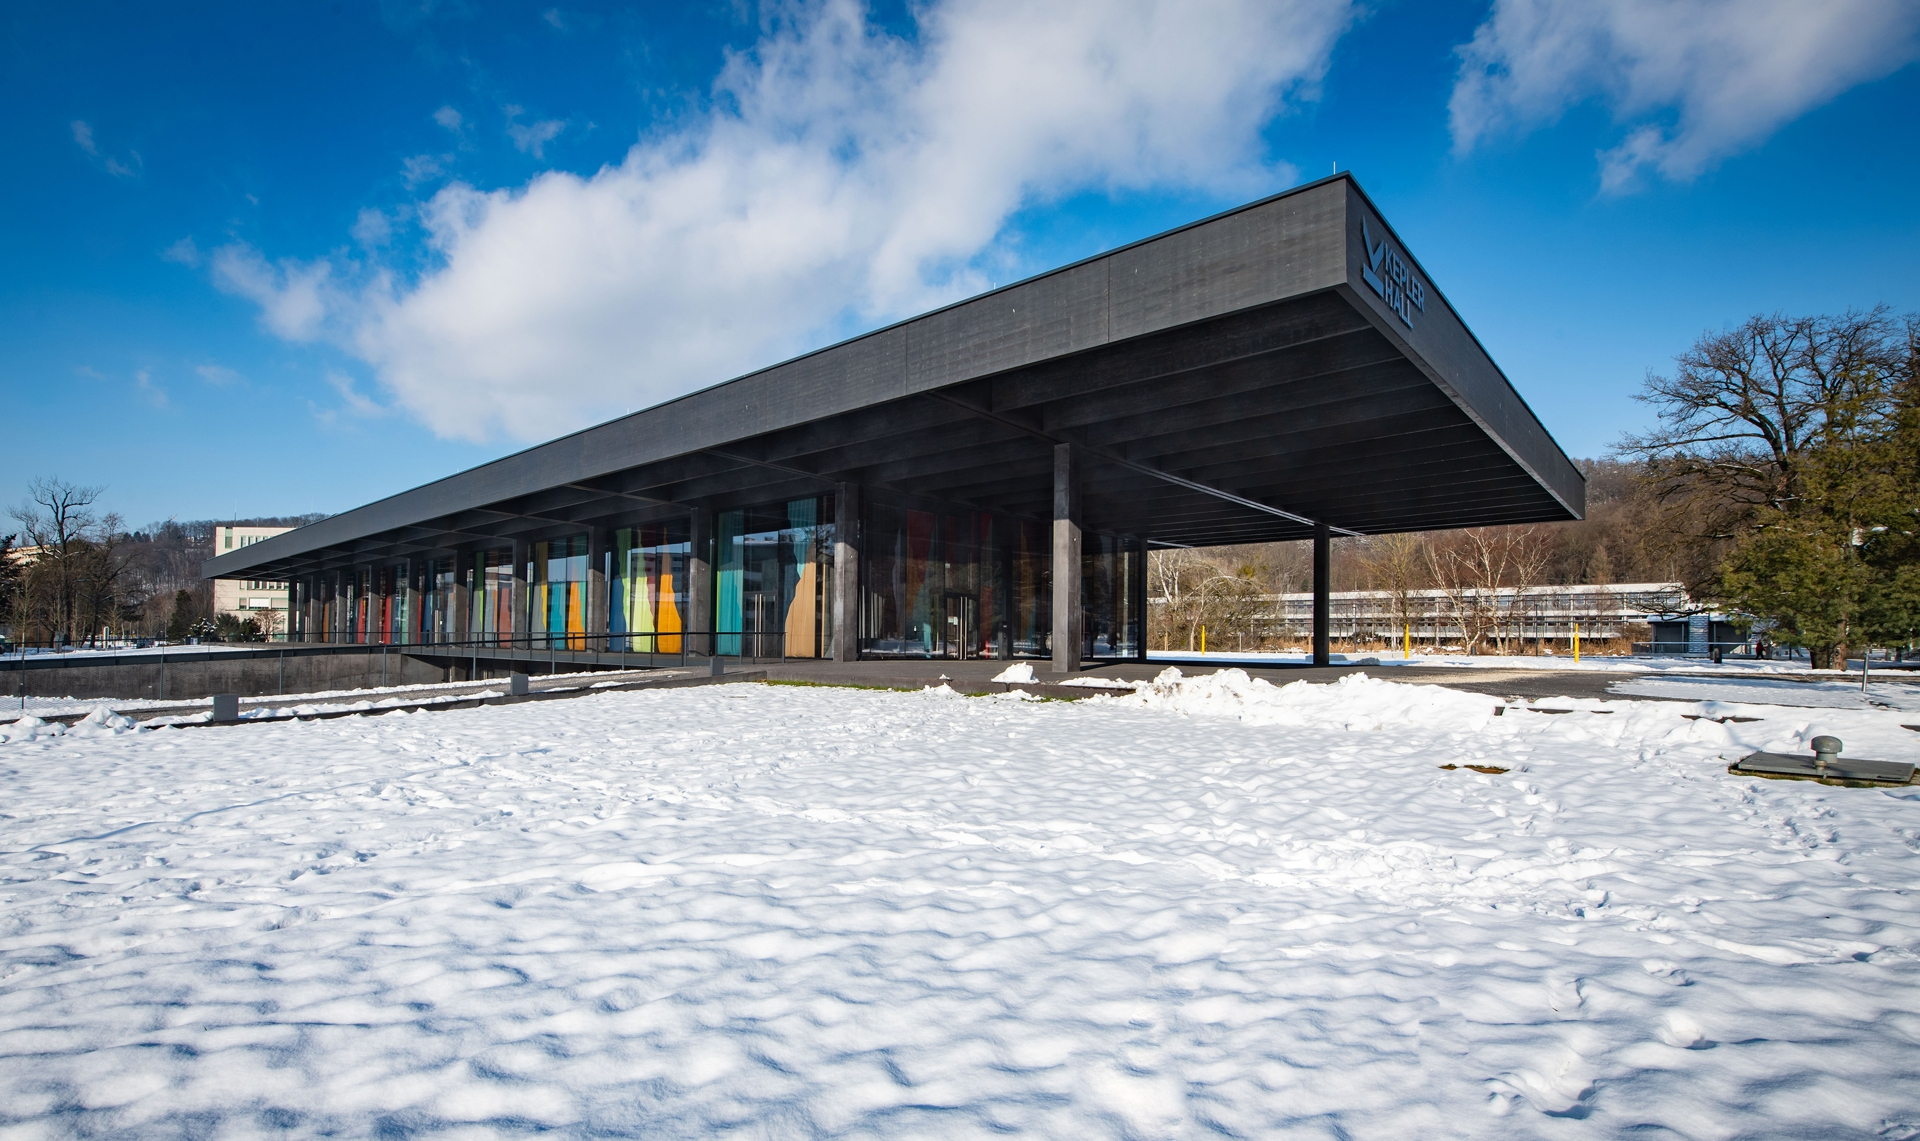
\includegraphics[width=\paperwidth]{images/jku_keplerhall_winter.jpg}}
%\setbeamercolor{normal text}{fg=white}
%\usebeamercolor[fg]{normal text}
%\begin{frame}[containsverbatim,plain]
%\frametitle{Background Image}
%
%You can add a full screen background image to a slide. The aspect ratio of the picture should match the presentation. To fill the whole screen you might use \verb|height=\paperheight|, but the result might be distorted~\ldots
%
%\bigskip
%\setbeamercolor{thisboxcolor}{bg=white,fg=black}
%\pgfsetfillopacity{0.6}
%\begin{beamercolorbox}[wd=\linewidth,dp=0ex,vmode]{thisboxcolor}
%\pgfsetfillopacity{1.0}
%\begin{lstlisting}[language={[LaTeX]TeX},numbers=none,xleftmargin=0.5em,xrightmargin=0.5em]
%\begingroup
%\usebackgroundtemplate{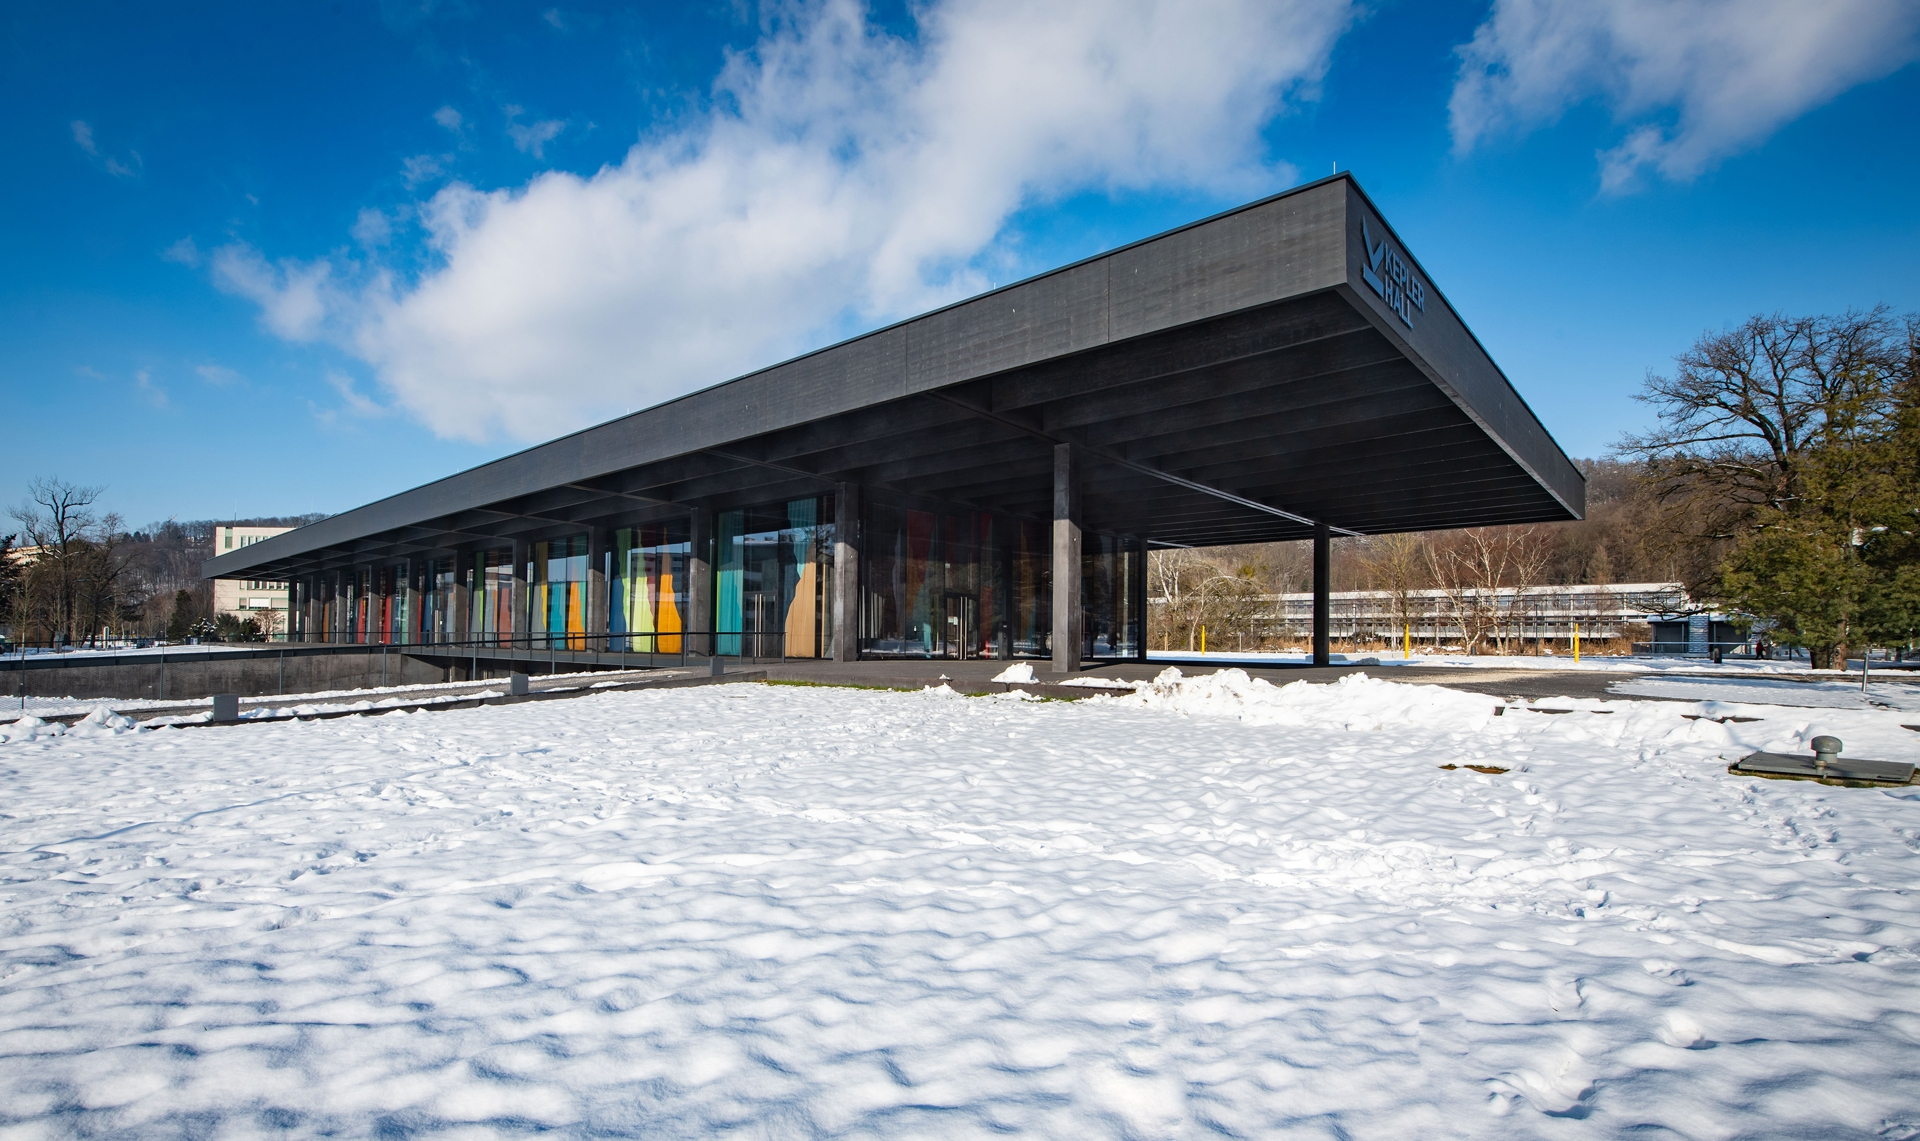
\includegraphics[width=\paperwidth]{images/jku_keplerhall_winter.jpg}}
%\setbeamercolor{normal text}{fg=white}
%\usebeamercolor[fg]{normal text}
%\begin{frame}[plain]
%\frametitle{Space for your frame title.}
%
%Space for your frame body.
%\end{frame}
%\endgroup
%\end{lstlisting}
%\end{beamercolorbox}
%\end{frame}
%\endgroup
%
%
%\begin{frame}[containsverbatim,plain]
%\frametitle{Title Image Slide}
%
%Use \verb|\imageframe[<mode options>]{<title>}{<subtitle>}{<graphic>}| to display a title image frame. That is a full screen image with a title sidebar.
%
%\begin{lstlisting}[language={[LaTeX]TeX},numbers=none]
%\imageframe{%
%    This is an image frame.
%}{%
%    With a subtitle.
%}{%
%    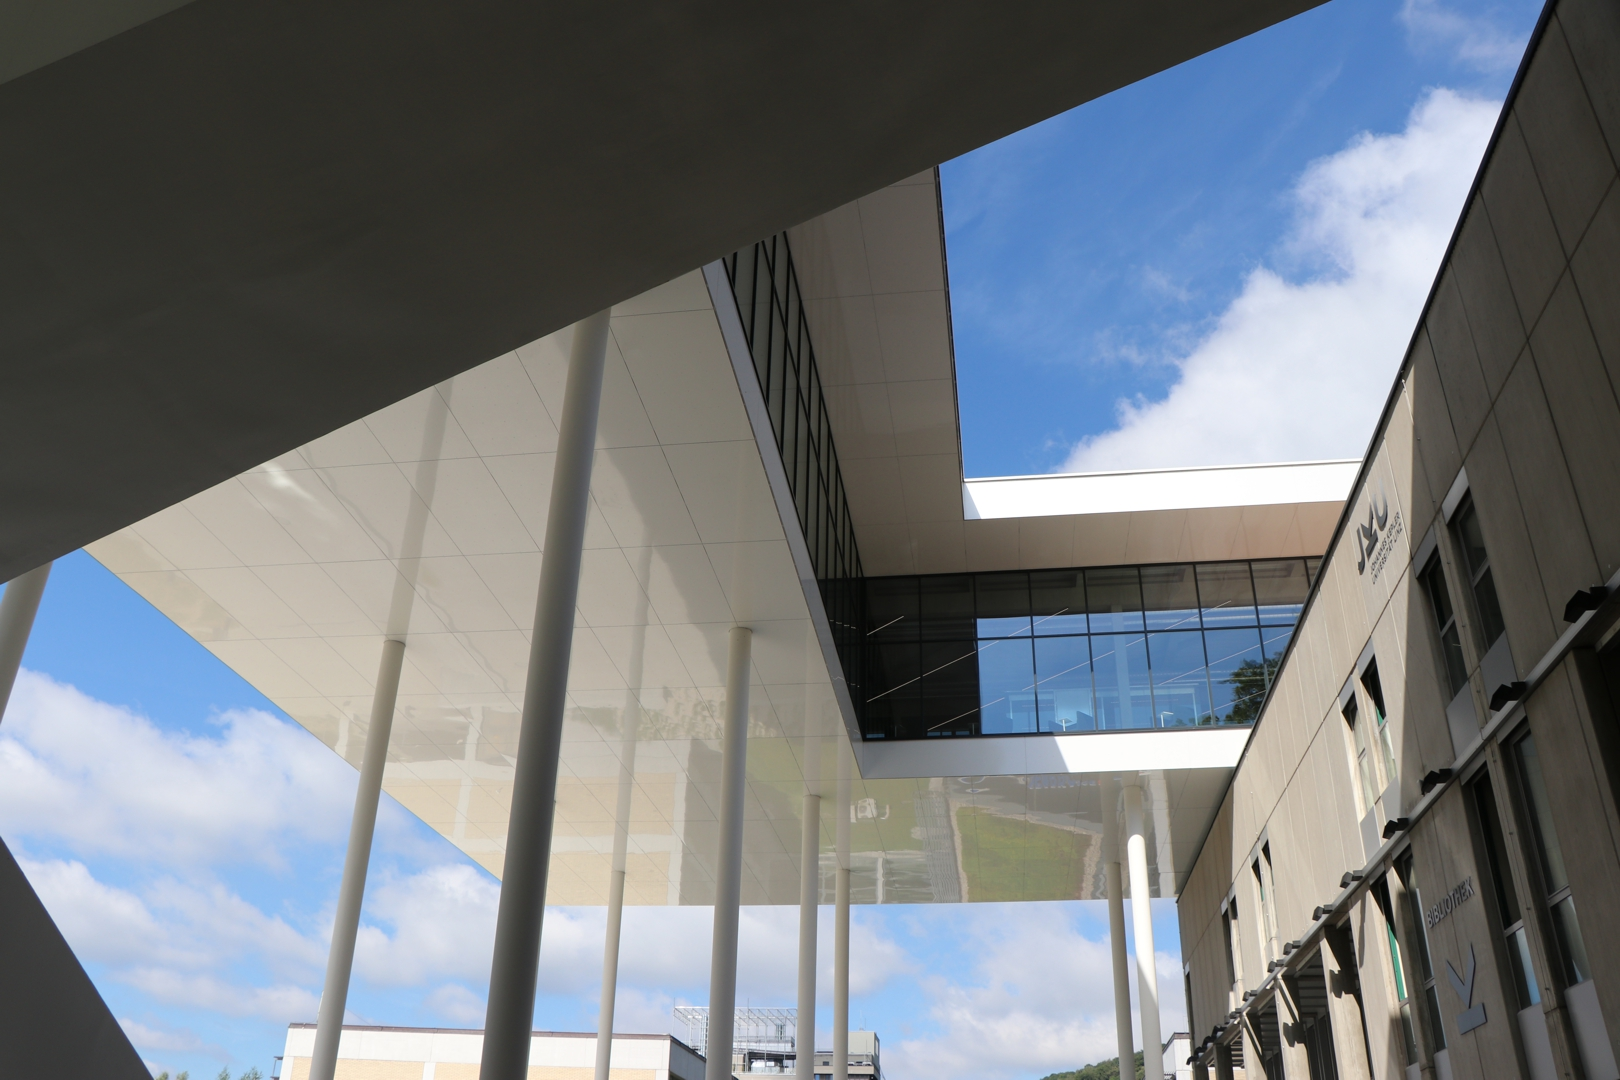
\includegraphics[height=\paperheight]{images/jku_learningcenter.jpg}
%}
%\end{lstlisting}
%
%The optional argument ``\textverb{<mode options>}'' may be any of the color mode options that can be used for the \verb|\maketitle| command (see slide~\ref{advanced-title-slides}).
%\end{frame}
%
%\imageframe[dark]{%
%    This is a title image frame.
%}{%
%    With a subtitle.
%}{%
%    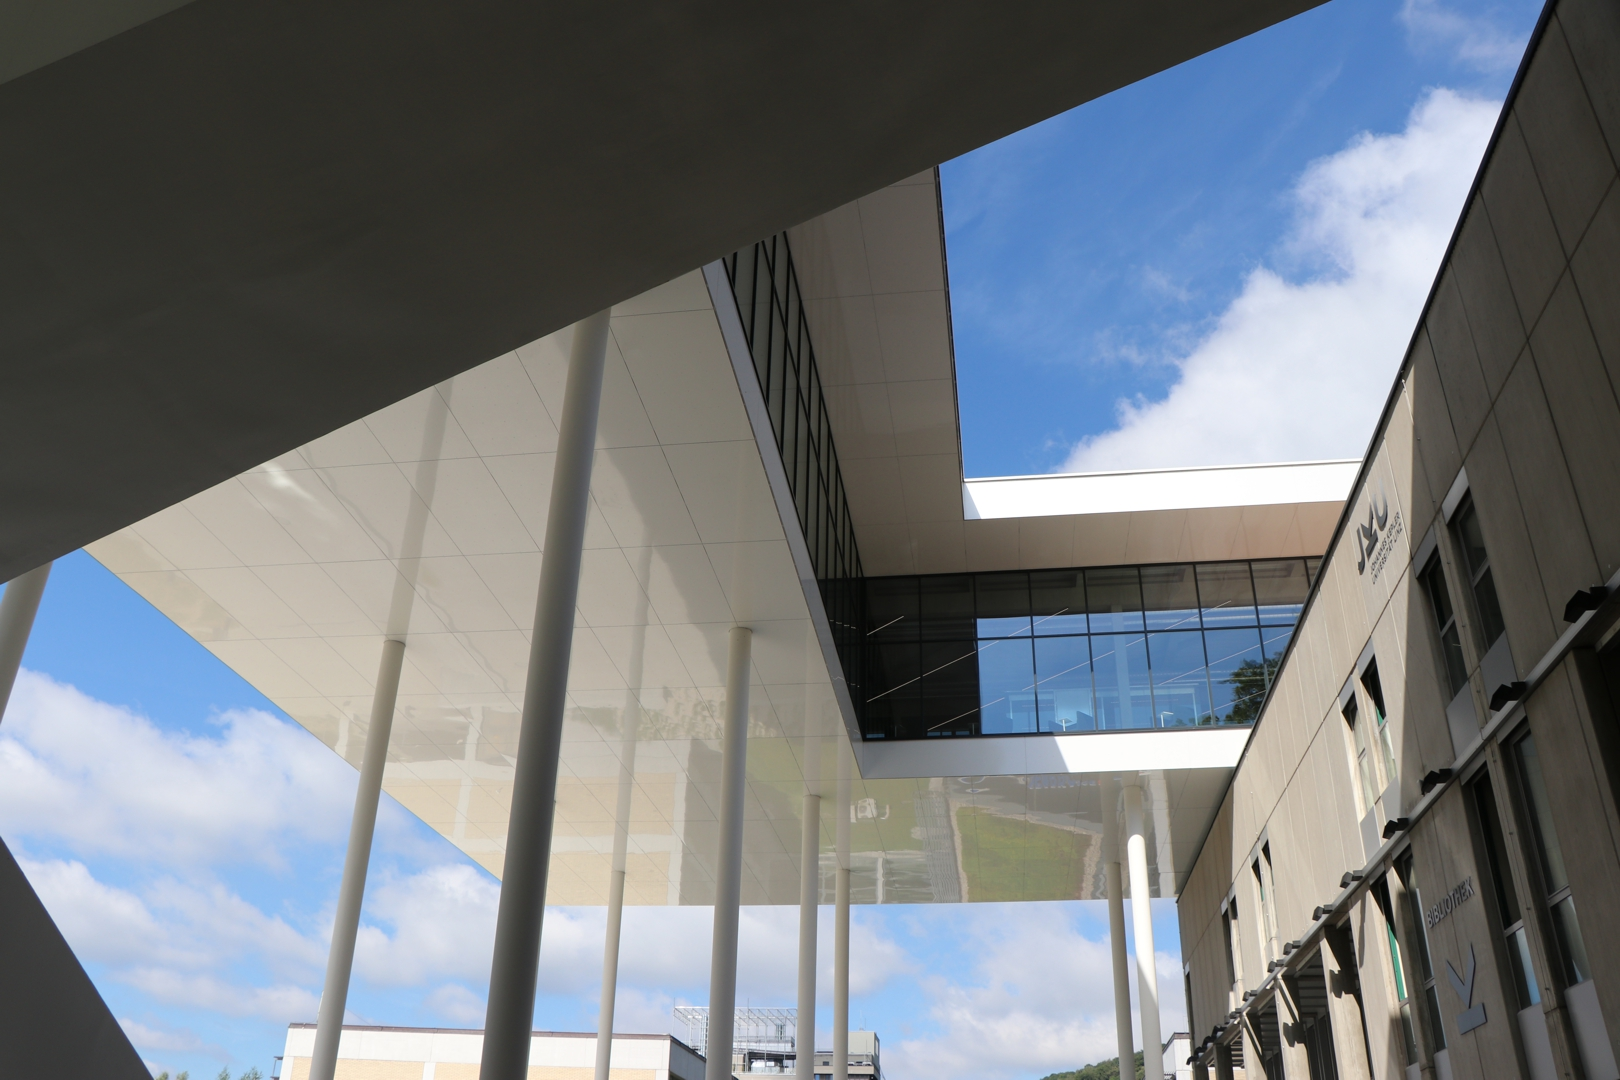
\includegraphics[height=\paperheight]{images/jku_learningcenter.jpg}
%}
%
%\imageframe[dark,MED]{%
%    This is a title image frame.
%}{%
%    For the MED faculty.
%}{%
%    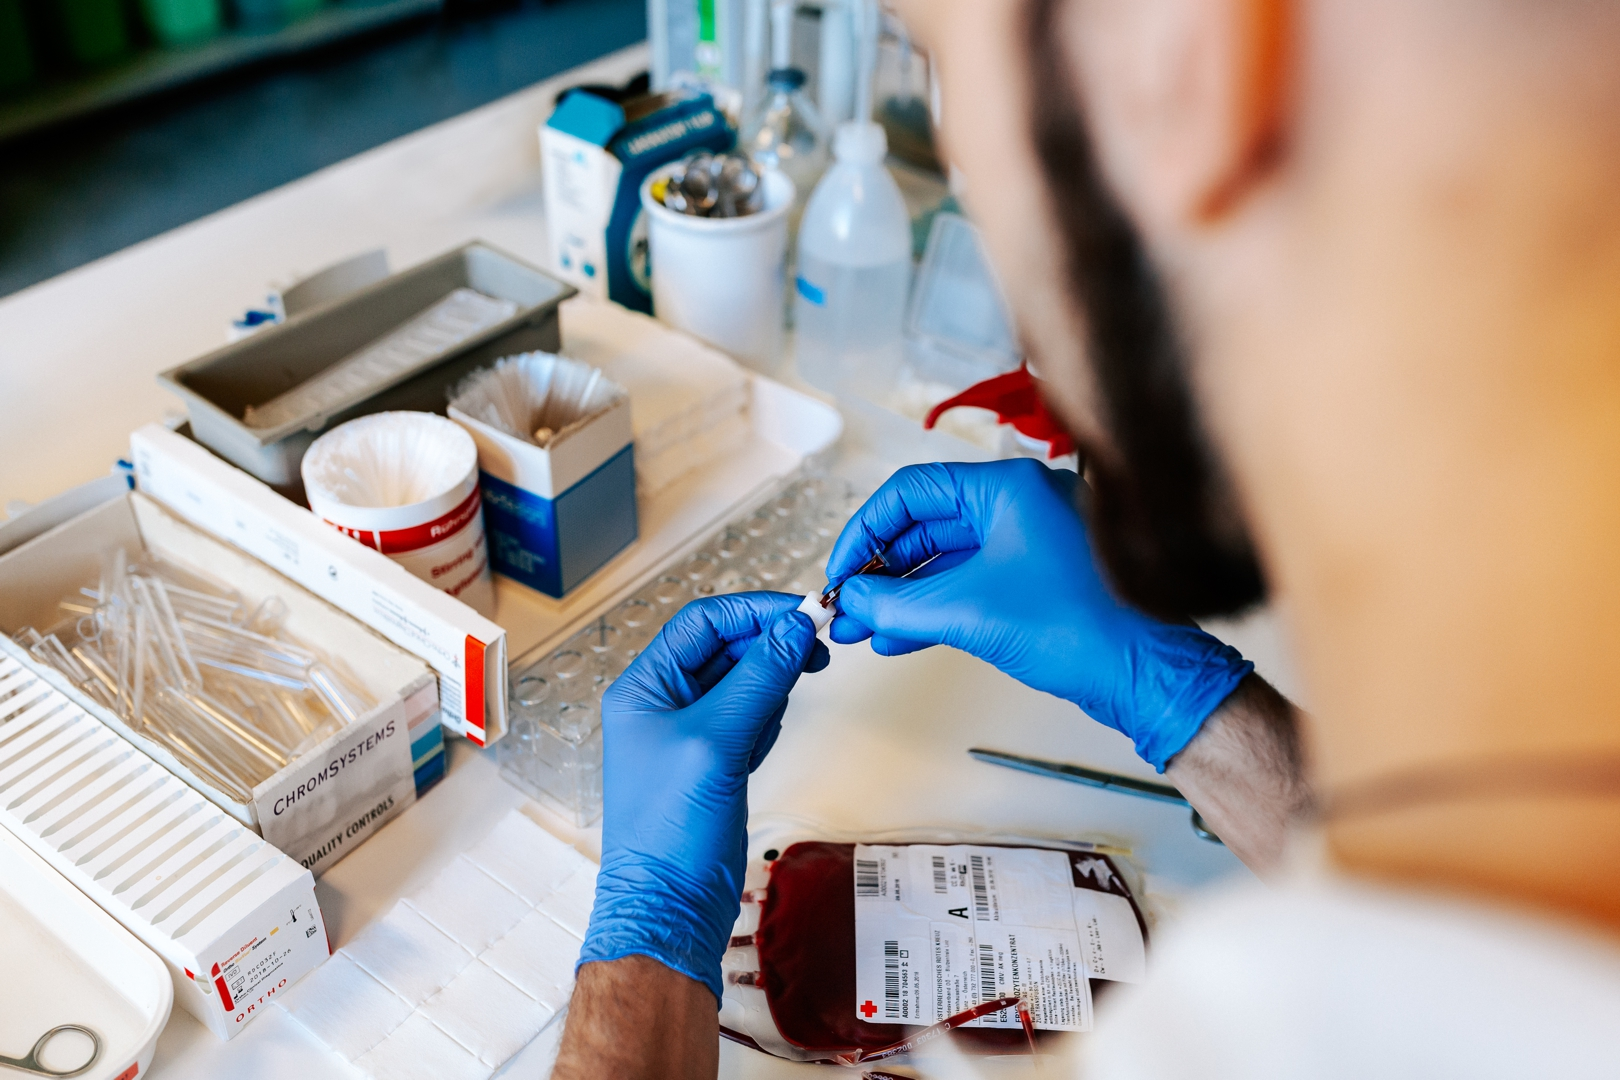
\includegraphics[height=\paperheight]{images/jku_med_image.jpg}
%}
%
%
%\begin{frame}[containsverbatim]
%\frametitle{Logo Slides}
%
%Use \verb|\jkulogo[<mode options>]| to display a logo slide. That is a slide with only the JKU logo centered on it. This slide is well suited as a final slide in your presentation.
%
%Again, the optional argument ``\textverb{<mode options>}'' may be any of the color mode options that can be used for the \verb|\maketitle| command (see slide~\ref{advanced-title-slides}), e.g.
%\begin{itemize}
%\item \textverb{\string\jkulogo}
%\item \textverb{\string\jkulogo[light]}
%\item \textverb{\string\jkulogo[dark]}
%\item \textverb{\string\jkulogo[SOWI,dark]}
%\item \textverb{\string\jkulogo[gray]}
%\item \textverb{\string\jkulogo[black]}
%\end{itemize}
%\end{frame}
%
%\jkulogo
%\jkulogo[light]
%\jkulogo[dark]
%\jkulogo[SOWI,dark]
%\jkulogo[gray]
%\jkulogo[black]
%
%
%\begin{frame}[containsverbatim]
%\frametitle{Switching Color Mode and Scheme}
%
%Just like switching the color mode and scheme for a specific special slide, you can also switch the color mode for the remaining part of the presentation. This may be useful if you want to create a presentation with parts focusing on more than one faculty.
%
%Use \verb|\setcolormode[<mode options>]| to change the color mode.
%\end{frame}
%
%
%\begin{frame}[containsverbatim,allowframebreaks]
%\frametitle{Contact Information Slide}
%
%Use \verb|\contactframe[<mode options>]{<name>}{<affiliation>}{<contact info>}{<ack>}| to display a contact information frame. 
%\begin{lstlisting}[language={[LaTeX]TeX},numbers=none]
%\contactframe{Johanna Kepler}{Institute of Networks and Security}{%
%    \contactphone{+43 732 2468-XXXX}
%    \contactmail{firstname.lastname@jku.at}
%    \contactweb[https://www.jku.at/ins]{jku.at/ins}
%}{%
%    This work is funded by XYZ.
%}
%\end{lstlisting}
%The optional argument ``\textverb{<mode options>}'' may be any of the color mode options that can be used for the \verb|\maketitle| command (see slide~\ref{advanced-title-slides}).
%
%\framebreak
%The contact info field may contain a combination of the following commands:
%\begin{itemize}
%\item \verb|\contactaddress{address}|: adds an address/place
%\item \verb|\contactphone{number}|: adds a phone number
%\item \verb|\contactfax{number}|: adds a fax number
%\item \verb|\contactmail{e-mail address}|: adds an e-mail address
%\item \verb|\contactweb[real url]{display url}|: adds a URL
%\item \verb|\contactother[icon]{contact info}|: adds an arbitrary contact info entry, use \verb|\fa...| (from \verb|fontawesome5| package) as icons
%\item \verb|\contactnewline|: adds an empty line
%\end{itemize}
%\end{frame}
%
%\contactframe[dark]{%
%    Johanna Kepler
%}{%
%    Institute of Networks and Security
%}{%
%    \contactphone{+43 732 2468-XXXX}
%    \contactmail{firstname.lastname@jku.at}
%    \contactweb[https://www.jku.at/ins]{jku.at/ins}
%}{%
%    This work is funded by XYZ.
%}
%
%\contactframe[light]{%
%    Johanna Kepler
%}{%
%    Institute of Networks and Security
%}{%
%    \contactphone{+43 732 2468-XXXX}
%    \contactmail{firstname.lastname@jku.at}
%    \contactweb[https://www.jku.at/ins]{jku.at/ins}
%}{%
%    This work is funded by XYZ.
%}
%
%
%
%
%
%
%\section{General \LaTeX/Beamer Features}
%
%
%\begin{frame}
%\frametitle{Environments}
%
%Standard \LaTeX-beamer defines several environments like
%\begin{quote}
%theorem, corollary, fact, lemma, problem, solution, definition, definitions, example, and examples.
%\end{quote}
%
%\begin{definition}[Monoid]
%We call $(M,\circ)$ a \emph{monoid} if and only if
%\begin{gather*}
%\forall a,b,c\in M:\quad(a\circ b)\circ c = a\circ(b\circ c) \tag{associativity}\\
%\exists e\in M \;\forall a\in M:\quad a\circ e = e\circ a= a \tag{neutral element}
%\end{gather*}
%\end{definition}
%\end{frame}
%
%\begin{frame}
%\frametitle{Environments}
%
%\begin{theorem}[Fundamental Theorem of \ldots]
%Let $(M,+)$ be a monoid. Then \ldots
%\end{theorem}
%
%\begin{proof}
%Let $M$ be an arbitrary set. We then show \ldots
%\end{proof}
%
%\begin{example}
%Put an example here.
%\end{example}
%\end{frame}
%
%
%\begin{frame}[fragile]
%\frametitle{Self-defined Environments}
%
%You also can define your own environments:
%\begin{lstlisting}[language={[LaTeX]TeX},numbers=none]
%\newtheorem{idea}[theorem]{Idea}
%
%\begin{idea}[My own idea]
%Here is a self-defined environment
%\end{idea}
%
%\theoremstyle{definition}
%\newtheorem{defi}[theorem]{My Definition}
%
%\begin{defi}
%Test
%\end{defi}
%\end{lstlisting}
%\end{frame}
%
%\newtheorem{idea}[theorem]{Idea}
%\theoremstyle{definition}
%\newtheorem{defi}[theorem]{My Definition}
%\theoremstyle{example}
%\newtheorem{ex}[theorem]{My Example}
%
%\begin{frame}[fragile]
%\frametitle{Self-defined Environments}
%
%\begin{idea}[My own idea]
%Here is a self-defined environment
%\end{idea}
%
%\begin{defi}
%Test
%\end{defi}
%
%\begin{ex}
%Test
%\end{ex}
%\end{frame}
%
%
%\begin{frame}[fragile]
%\frametitle{Custom Blocks}
%\begingroup
%\setbeamercolor{block title}{fg=white,bg=jkuBlue}
%\begin{block}{Blue block}
%Using the theme colors to generate colored blocks.
%\end{block}
%\endgroup
%
%\begin{lstlisting}[language={[LaTeX]TeX},numbers=none]
%\begingroup
%\setbeamercolor{block title}{fg=white,bg=jkuBlue}
%\begin{block}{Blue block}
%Use the theme colors to generate colorful blocks.
%\end{block}
%\endgroup
%\end{lstlisting}
%\end{frame}
%
%
%\begin{otherlanguage}{ngerman}
%\begin{frame}[fragile]
%\frametitle{Language}
%\begin{itemize}
%\item Use the \textverb{otherlanguage} environment to temporarily change the document language in your presentation.
%\item Changing the document language to \textverb{german} (or better \textverb{ngerman}) also changes the language in logos and the imprint on title pages and in footers.
%\end{itemize}
%
%\begin{lstlisting}[language={[LaTeX]TeX},numbers=none]
%\begin{otherlanguage}{ngerman}
%
%\end{otherlanguage}
%\end{lstlisting}
%\end{frame}
%\end{otherlanguage}
%
%
%\begin{frame}[label=handout]
%\frametitle{Producing Handouts}
%
%\begin{itemize}
%\item You can generate a ``handout'' version of your presentation with the class option \textverb{handout}.
%\item Section slides and logo slides will be suppressed.
%\item Overlays will be flattened into single pages.
%\item Slide numbering will still match the numbering in the non-handout version.
%\end{itemize}
%\end{frame}
%
%
%\section{Ending the Presentation}
%
%\begin{frame}
%\frametitle{Thank You Thank You Thank You Thank You Thank You Thank You Thank You Thank You Thank You}
%
%You see, btw., the slide title can run over several lines \ldots
%
%\bigskip
%\begin{alertblock}{Please \ldots}
%\ldots\ refrain from putting an extra slide at the end saying ``\alert{Thank you for your attention}''. This is really annoying~\cite{schultz,karol}. You can say ``Thank you'' anyway, it need not be written. Instead, you can put a nice \textverb{\string\jkulogo} as the final slide!
%\end{alertblock}
%
%\end{frame}
%
%
%\begin{frame}[allowframebreaks]{References}
%%\setbeamerfont{bibliography item}{size={\footnotesize}}
%%\AtNextBibliography{\footnotesize}
%\printbibliography
%\end{frame}
%
%
%\begin{frame}
%\frametitle{JKU Theme Information}
%
%This a beamer theme for \href{https://www.jku.at/}{Johannes Kepler University Linz, Austria}.
%
%\bigskip
%\begin{exampleblock}{Want to report a bug? Want to request improvements?}
%You are always welcome to suggest improvements via the official repository at \url{https://github.com/michaelroland/jku-templates-presentation-latex}.
%\end{exampleblock}
%\end{frame}
%
%
%\jkulogo

\end{document}
\endinput
